% REMEMBER: You must not plagiarise anything in your report. Be extremely careful.
\documentclass{l4proj}

    
%==============================================================================
% Put any additional packages here
\usepackage{wrapfig}
\usepackage{graphicx}
\usepackage{tabularx}
\hypersetup{
    colorlinks=true,
    linkcolor=black,
    filecolor=magenta,      
    urlcolor=blue,
    citecolor=black
}
% You can add any packages you want, as long as it does not alter
% the overall format (e.g. don't change the margins or the reference style).
%
\usepackage{pdfpages} % if you want to include a PDF for an ethics checklist, for example
%
%

\begin{document}

%==============================================================================
%% METADATA
\title{SmartPeerJS: A library for turning smartphone in interactive controller} % change this to your title
\author{Emma Poliakova}
\date{March 31, 2022}

\maketitle

%==============================================================================
%% ABSTRACT
\begin{abstract}
     Smartphones are small, convenient and powerful devices almost all of us have. They are packed full of sensors that go beyond making a phone call or social network scrolling. This project aims to provide and demonstrate a simple way of turning smartphones into various controllers and using them to perform actions in a computer browser. All it takes is a single QR code to start a peer-to-peer connection, no extra software installations required.  An open-source library has been created to facilitate this connection and to allow for easy creation of new controllers. It only takes two lines of code to get started and the library offers many functionalities including QR code generation and statistics calculation. The evaluation has shown that the ping rate is low, therefore there is little lag but the polling rate is only about half compared to conventional controllers. The user interview revealed that the library is easy to use and integrates well with games.
\end{abstract}

%==============================================================================
%% ACKNOWLEDGEMENTS
\chapter*{Acknowledgements}
% Enter any acknowledgements here. This is optional; you may leave this blank if you wish,
% or remove the entire chapter
%
% We give thanks to the Gods of LaTeX, who in their eternal graciousness, 
% have granted that this document may compile without errors or overfull hboxes.
%

%==============================================================================

% EDUCATION REUSE CONSENT FORM
% If you consent to your project being shown to future students for educational purposes
% then insert your name and the date below to  sign the education use form that appears in the front of the document. 
% You must explicitly give consent if you wish to do so.
% If you sign, your project may be included in the Hall of Fame if it scores particularly highly.
%
% Please note that you are under no obligation to sign 
% this declaration, but doing so would help future students.
%
\def\consentname {Emma Poliakova} % your full name
\def\consentdate {31 March 2022} % the date you agree
%
\educationalconsent


%==============================================================================
\tableofcontents

%==============================================================================
%% Notes on formatting
%==============================================================================
% The first page, abstract and table of contents are numbered using Roman numerals and are not
% included in the page count. 
%
% From now on pages are numbered
% using Arabic numerals. Therefore, immediately after the first call to \chapter we need the call
% \pagenumbering{arabic} and this should be called once only in the document. 
%
%
% The first Chapter should then be on page 1. 

% PAGE LIMITS
% You are allowed 40 pages for a 40 credit project and 30 pages for a 
% 20 credit report. 
% This includes everything numbered in Arabic numerals (excluding front matter) up
% to but *excluding the appendices and bibliography*.
%
% FORMATTING
% You must not alter text size (it is currently 10pt) or alter margins or spacing.
% Do not alter the bibliography style. 
%
%==================================================================================================================================
%
% IMPORTANT
% The chapter headings and structure here are **suggestions**. You don't have to follow this model if
% it doesn't fit your project. Every project should have an introduction and conclusion,
% however.  If in doubt, your supervisor can give you specific guidance; their view takes precedence over
% the structure suggested here.
%
%==================================================================================================================================
\chapter{Introduction}

% reset page numbering. Don't remove this!
\pagenumbering{arabic} 

% You can use \todo{} to mark text that needs to be fixed. Anything inside will appear as highlighted 
% text in the final copy, and you will also get warnings when you compile (so you don't
% forget to take them out!)

\section{Motivation}

Almost everyone owns a smartphone nowadays. Current smartphones are essentially small portable computers, offering a large array of sensors, such as cameras, microphones, accelerometers, and touchscreens. They are powerful, inexpensive devices capable of performing countless actions. Most of the time, however, their potential is overlooked and they are used solely for social media and calls.  \par

On the other hand, we have expensive devices designed for a single purpose. This could be equipment dedicated to hand or eye-tracking, a game console controller, or a steering wheel for racing games. Due to their cost and narrow range of applications, they can be inaccessible to most people. Instead, harnessing the potential offered by smartphones can offer much of the same functionality while being widely accessible to the public. Smartphones can be used to create various controllers while avoiding the need for any expensive gadgets or software installations. \par

The idea behind this project is to utilize the capabilities of a smartphone and turn it into a controller such as a joystick, NES controller, or hand tracker among others, by scanning just a single QR code. All the communication would take place in a browser; thus bypassing the need to download or install any software. Every game, demo, and web application could have its own, unique controller. As such, users would no longer be restricted by having to purchase different controllers to try out new technologies. \par 

This project aims to offer tools in the form of an open-source library that will facilitate the easy creation of such smartphone controllers. The data stream between the smartphone and the computer would be managed automatically, allowing users to apply this technology to make any interactive web application or controller they want, without having to worry about creating the connection between the devices first. 

\section{Goals}

\textbf{Provide easy peer-to-peer connection} \par
The overall goal of the project is to create an open-source library that will establish a peer-to-peer connection between a computer browser and a smartphone browser in just a few lines of code. An object that handles the connection would be the base of every controller offered in this library. This setup would also allow for the creation of new controllers without requiring the user to know anything about, or work with, Web Real-Time Communication - WebRTC and the connection itself. \par

\textbf{Use of smartphone sensors}\par
There are countless options for controllers that can be made using smartphone sensors. A microphone could be used for a voice-controlled application, a video stream could be sent to a browser for object recognition. The focus will first be on using the touchscreen, and future expansions to other sensors should be made easily realizable. \par

\textbf{Data management}\par 
The open-source library should be structured into multiple classes, each class managing a different type of controller data. For example, a dedicated class to manage the information provided from a joystick and a different class to store data from an NES controller. \par

\textbf{Supporting multiple controllers}\par
 The library will offer some finished, ready-to-use controllers and the user can also make their own without having to modify any of the core code. The structure of the library should provide a clear way of integrating new controller classes for anyone who wishes to contribute to the repository. \par
 
\textbf{Multiplayer}\par
The library should support multiplayer games naturally. The user will not need to specify beforehand how many peer connections they will use. It will be easy to add new connections at any point and disconnections are going to be handled automatically.  \par

\textbf{Easy to integrate with games}\par
Accessing the data from the smartphone needs to be easy and straightforward. If using a dedicated controller class, for example, a class for a joystick, the class fields should be descriptive. There should also be a clear way of distinguishing between the players. \par

\textbf{Users should not be required to set up a server}\par 
Once the peer-to-peer connection is established, the project can run without a server. It is therefore completely free to run on any computer or smartphone. All controllers and demos can be hosted on GitHub, such that they are available at all times. The initial connection that does need a server is handled by PeerJS and WebRTC, and no networking knowledge is necessary from users. 

\textbf{Provide clear and concise documentation}\par
The key to the success of an open-source library is providing good quality guidance for new users who wish to utilize or even contribute to the project. This means writing documentation that is sufficiently detailed to explain the use cases, but not too long or dense, which may put potential users off trying it out. 

\textbf{Publish on npm}\par
Finally, the library should be published on Node package manager npm. Npm became the main package manager for JavaScript projects and it makes it easy to install the available packages. Furthermore, publishing on npm will make the source code visible to other content delivery networks such as UNPKG meaning the user does not have to install the package directly if they do not wish to.





%==================================================================================================================================
\chapter{Background}

\section{Open-source library}
An open-source library is a collection of reusable files that can be integrated with projects. It eliminates the need to code frequently used resources every time they are required. The key features of an open-source library are that it is free to reuse, modify and publish without permission \cite{HeavyAI}. The idea of open-source free software has been around since the 1950s, the software being shared mainly among researchers at various universities \cite{spice}. The popularity of free and open-source started increasing in the 1980s and 1990s with the release of Linux operating system in 1991 contributing to the free software movement \cite{mob}. At present, open-source libraries became a major part of software development. Among the most famous are React, TensorFlow, Django, Next.js, and many more. When a library is freely available, it allows to speed up the development process of other projects. It also makes the code itself more efficient as the large-scale libraries, for example, React mentioned above or EventEmitter, are usually developed by teams of programmers and go through rigorous testing and optimization. 

\section{Web Real-Time Communication}
The key element of the project is the use of Web Real-Time Communication or Web This allows the communication between browsers without the need of an intermediary \cite{rtc}. WebRTC is used to establish peer-to-peer (P2P) communication and allows to share video, audio, and generic data. Many popular applications are built with WebRTC such as Discord, Snapchat, WhatsApp, and Facebook Messenger \cite{rtc_use}. \par
WebRTC enables peer-to-peer communication but still needs servers for the initial set-up. These are signaling server, STUN, and TURN servers. \cite{rtc_infra}. The infrastructure is shown in figure \ref{fig:webrtc}. The signaling server allows two peers to "find each other". If peer 1 wishes to start a communication channel with peer 2, it creates an offer in the form of session description protocol (SDP) and sends it to the signaling server. Peer 2 can read the offer from the server and create an SDP answer which is also passed to the signaling server.\cite{rtc_in_100}. \par 
STUN and TURN are a part of the signaling process and are built in the WebRTC API. If the peer-to-peer connection is to be established, then there is a need for a unique identifier which in this case is the IP address. Most devices are hidden behind firewalls and their IP addresses constantly change because of NAT - network address translation. \cite{stun_turn}. However, without a public address we cannot have P2P. The STUN server is responsible for finding out the public IP addresses of the two peers. \cite{rtc_infra}. \par
TURN is essentially a backup for STUN. When it is impossible to find out the real IP address, the TURN server is used to reroute the messages between the peers. \cite{server} In other words, the server relays the data between the peers when STUN could not provide direct P2P. 



\begin{figure}[h!]
    \centering
    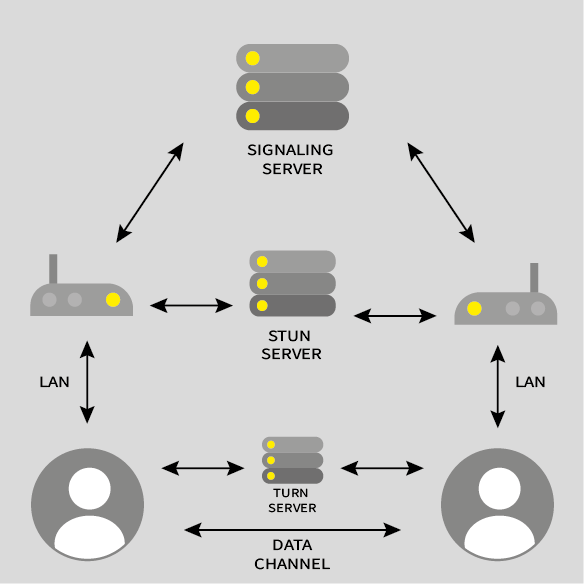
\includegraphics[width=10cm]{./images/webrtc.png}
    \caption{WebRTC infrastructure, adapted from \cite{server}}
    \label{fig:webrtc}
\end{figure}

\section{Node package manager - npm}
Npm is the world's largest software registry, it contains almost two million packages. \cite{npm}. It is a way for developers to share open-source code. Many JavaScript applications are built with the use of npm packages, some of the most frequently used modules include React, Angular and, jQuery. Npm offers packages for a wide range of problems, starting with small helpful maths functions to full frameworks. The areas covered include CSS, robotics, coverage and, testing. Releasing a package to npm makes it more convenient and accessible to programmers and helps to advertise the library. The npm packages can be installed directly through the command line. Once the package is published, it can also be included in a project with a single URL.

\section{Existing products}
To my best knowledge, the only similar open-source library focused on turning smartphones into different controllers and connecting them to a computer browser is called \href{https://github.com/snex-io/snex-lib}{Snex.io}. The library focuses exclusively on retro controllers but uses the same principle as my library to establish the connection. However, the Github repository shows it has been inactive since 2018 and the official website has recently been disabled. I discovered this library while already working on my project, therefore the main source of inspiration for this project was other products. The two major ones are the Leap Motion controller and Makey Makey kit. 

\subsection{Leap Motion Controller}
A Leap Motion controller is a device that supports hands and finger motions as input to replace a computer mouse. It requires no touching and it captures the hand movements with high accuracy. \cite{leap}. It is an interesting piece of equipment, however, its costs around £80 and therefore, it is not accessible to the wider public. It provided great inspiration in the initial stages of my project. While it is hard to match in accuracy, the use of smartphones could significantly boost accessibility.

\begin{figure}[h!]
    \centering
    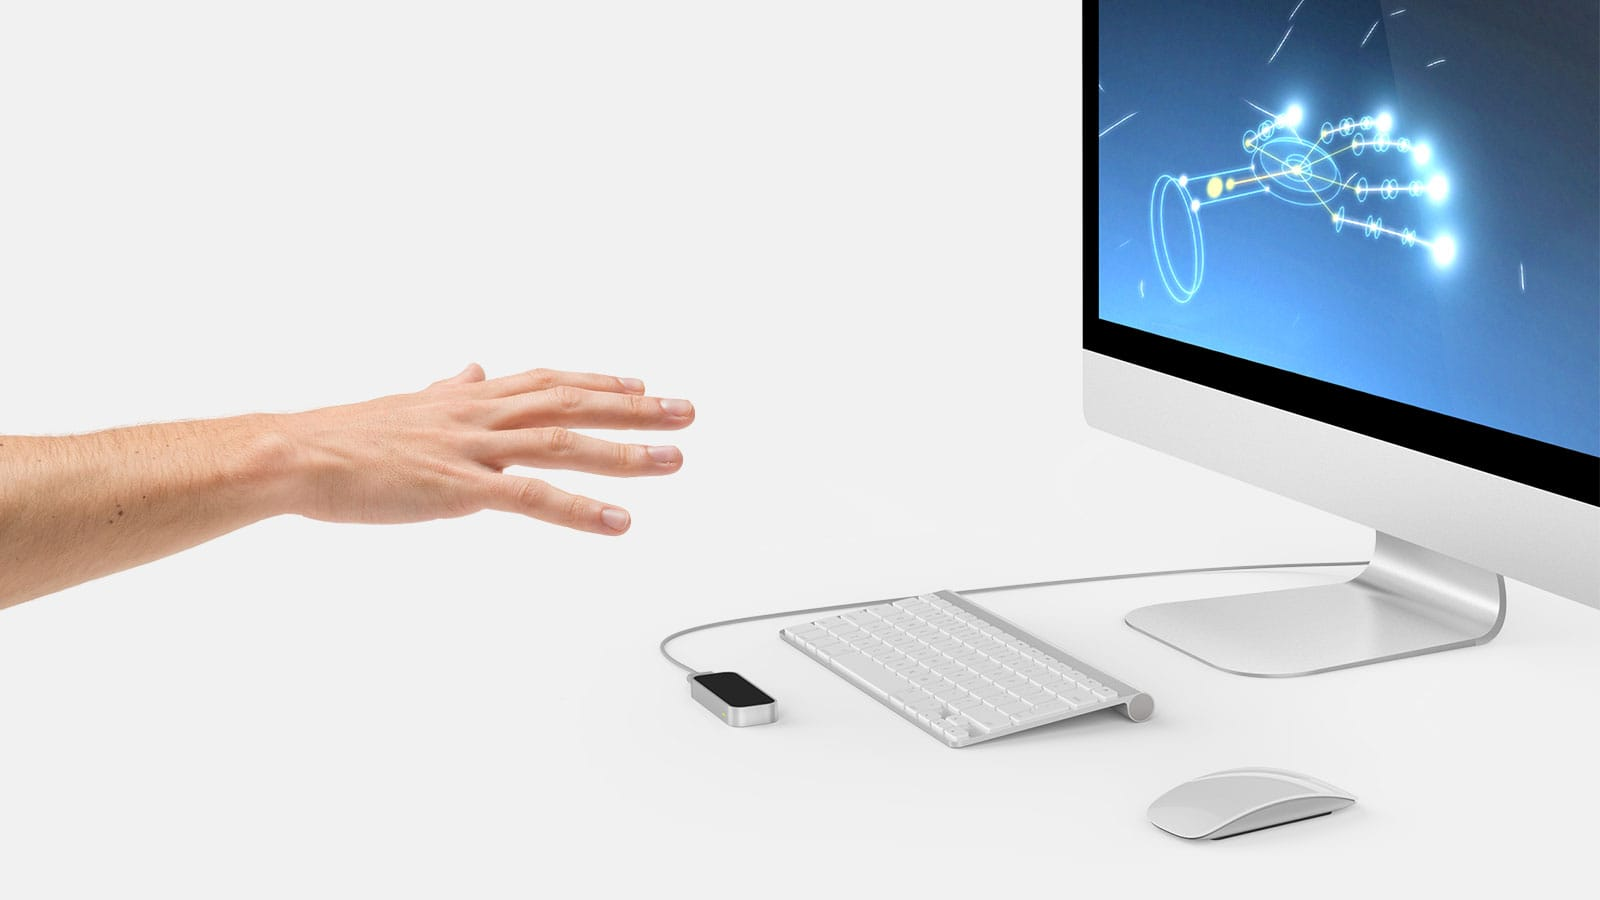
\includegraphics[width=7cm]{./images/leap.jpg}
    \caption{\cite{leap_pic}}
    \label{fig:leap}
\end{figure}

\subsection{Makey-Makey}
Makey-Makey is an invention kit consisting of a circuit board, alligator clips, and a USB cable. It allows everyday objects to be turned into computer keys and hence control any computer program or webpage that accepts keyboard and mouse clicks. \cite{makey}. It is a playful way of teaching coding by letting people create controllers from ordinary things. For example, it lets the user turn bananas into keyboard keys. Once again, the price of this kit is around £50 which could pose a problem, especially for a larger group.  

\begin{figure}[h!]
    \centering
    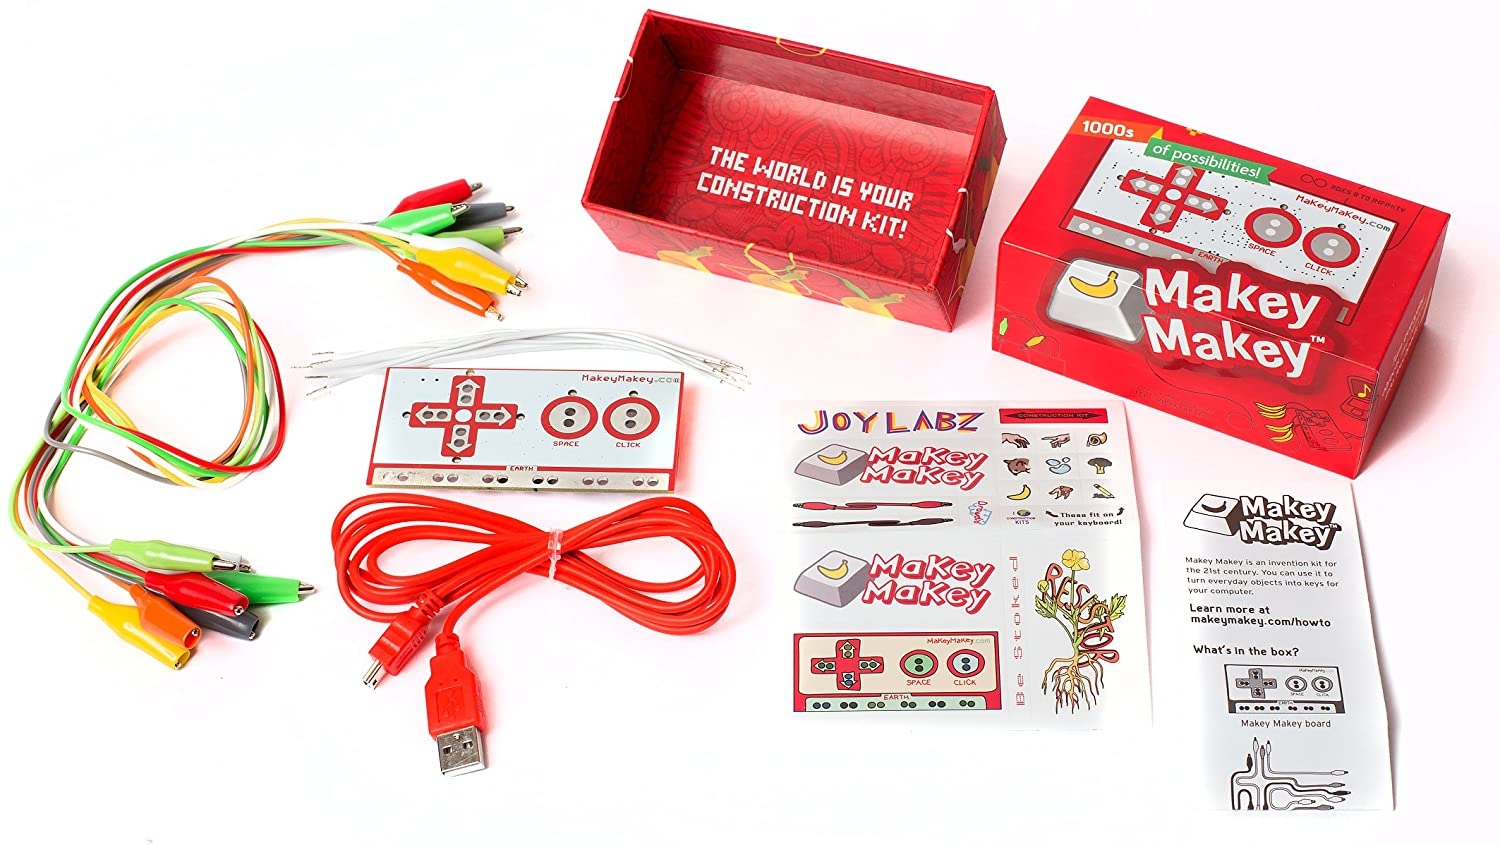
\includegraphics[width=7cm]{./images/makey.jpg}
    \caption{\cite{makey_pic}}
    \label{fig:makey}
\end{figure}


\section{Summer internship}
These products along with WebRTC technology inspired my summer internship project at the University of Glasgow. The initial goal was to replicate parts of the Leap motion sensor and Makey-Makey kit using only a smartphone and create basic demos where a computer browser would be controlled by input from a smartphone. It would use the smartphone camera to stream video to the computer browser which could then be used for hand tracking or object recognition. Therefore, this technology would be available to anyone with a smartphone and an Internet connection for free. The second main point was to ensure no extra software installation is needed. To make this possible, the communication between the phone and the computer is established through browsers and WebRTC. Once the connection was established the video input could be used to control the computer screen or perform some actions. 

\subsection{Hand tracking}
The first library used to provide hand tracking was \href{https://google.github.io/mediapipe/solutions/hands.html}{Google's MediaPipe}. However, it only supported direct webcam input and not a video stream sent from a smartphone. I decided to switch to a library called \href{https://github.com/tensorflow/tfjs-models/tree/master/handpose}{Handpose}. The hand tracking system is very similar to MediaPipe while accepting a larger variety of video inputs. I was able to create a basic hand tracker. It allowed the user to scan a QR code with their smartphone to start a video stream. The computer browser would then apply the hand tracking algorithm to the video input and use the index finger coordinates to move a ball on canvas. 

\begin{figure}[h!]
    \centering
    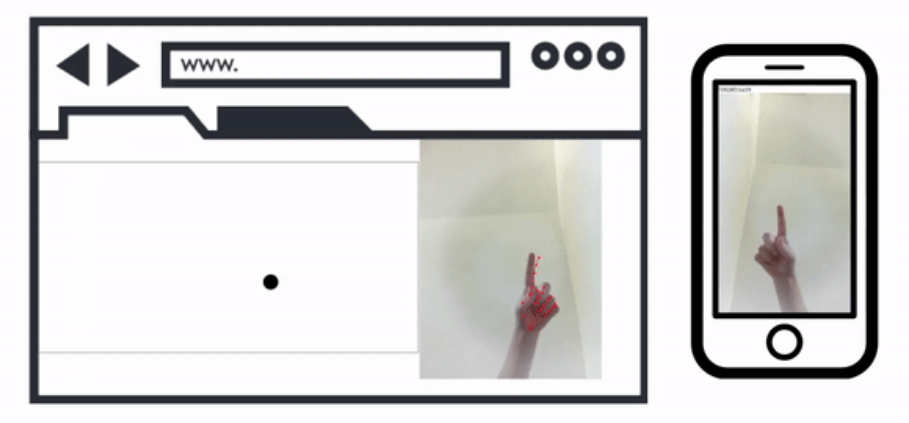
\includegraphics[width=10cm]{./images/hand.png}
    \caption{Hand tracking demo}
    \label{fig:hand}
\end{figure}

\subsubsection{Issues}
There were multiple issues with the hand tracking demo which lead to switching the project's focus to different sensors provided by the smartphone, mainly the touchscreen. The main problem for hand tracking was the loading time, it would take up to several minutes to initialize. To show the user that the hand is being recognized the browser displayed the smartphone video with a hand graph drawn over it. This led to another issue when the graph would occasionally freeze making the response slow. \par
The second main problem was the distance needed to cover the entire canvas. The user would need to stand far away from the phone to be able to use their hand to move the ball around the full size of the canvas. The attempted solution to this problem was attaching a wide-angle lens to the smartphone. However, this did not make a big enough difference and it would take away from the idea of not needing any extra equipment.

\begin{figure}[h!]
    \centering
    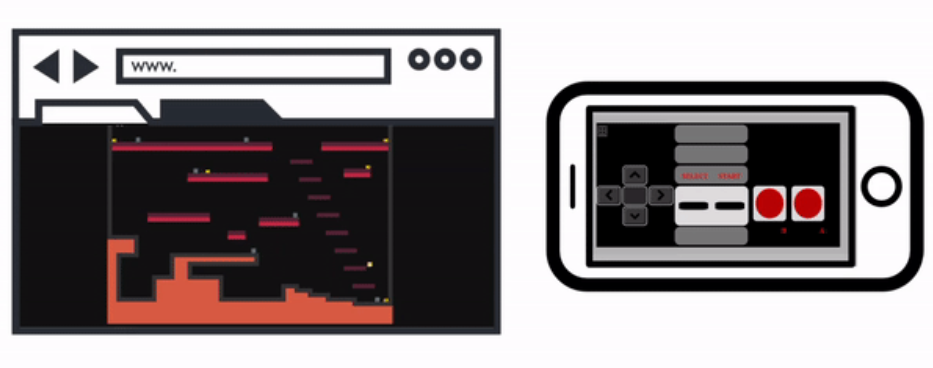
\includegraphics[width=10cm]{./images/demo2.png}
    \caption{Platformer demo}
    \label{fig:platform}
\end{figure}

\subsection{Game demos}
The focus of the project shifted to the touchscreen as an input to the computer browser. The advantages were the ease of use and instant availability. The rest of the internship was centered around converting existing JavaScript games to work with touchscreen input rather than a standard keyboard and mouse. I developed three controllers: joystick, NES controller, and plain touchpad which uses canvas to capture the tap coordinates. I then converted a racing game and a platformer to be used with a smartphone while the game is displayed on a PC screen. I created a basic block-stacking simulator that uses a physics engine. The player can use the entire touchscreen to pick up objects on the computer screen and stack them. The demos were a great source for creating user tutorials later in the project.


\subsection{Conversion to open source library}
With many working demos, a pattern started to appear. Each website would first initialize a peer. Then multiple event listeners were created, waiting for connection from a smartphone, then incoming data, and finally a disconnection. This showed that the code could be packaged into modules to allow other users to create their own games and controllers. Especially with the variety of sensors a smartphone has to offer, the library would have the potential to attract many creative projects. The last two weeks of the internship were dedicated to planning out the process and steps needed to move from the proof of concept demos to an open-source library. This included researching Node.js, Webpack, looking at examples of other open-source libraries to figure out the structure and organization. By the end of the internship, I had created a \href{https://github.com/EmmaPoliakova/WebRTCSmartphoneController}{portfolio} which explained the basic logic behind the project and showcased five different demos: a racing game with a joystick, a platformer with an NES controller, a single-player and a multiplayer stacking simulator with a touchpad and a hand tracking game with a smartphone camera. On top of that, I had the first proposal for the future open-source library structure.

%==================================================================================================================================
\chapter{Analysis/Requirements}
This chapter discusses the functional and non-functional requirements. Some of them were identified at the end of the summer internship while others emerged during the planning of the project.

\section{Problem specification}
The figure \ref{fig:libstruct} demonstrates the initial requirements planned out at the end of the summer internship. It shows the basic structure of the library as well as required features. During the course of the project, the classes have been renamed but the concept stayed the same. At the centre of the library is PeerJS which facilitates peer-to-peer connection. The class in the blue frame is directly interacting with PeerJS and acts as a data manager for all the incoming data messages and well as an event handler. The green frame represents specific controller classes. These allow to store different data types each controller requires. For example, a joystick class would store the angle of the joystick while a touchpad class would keep all the coordinate pairs for fingers. Finally, instances of green classes can be created to support different games and web applications.

\begin{figure}[h!]
    \centering
    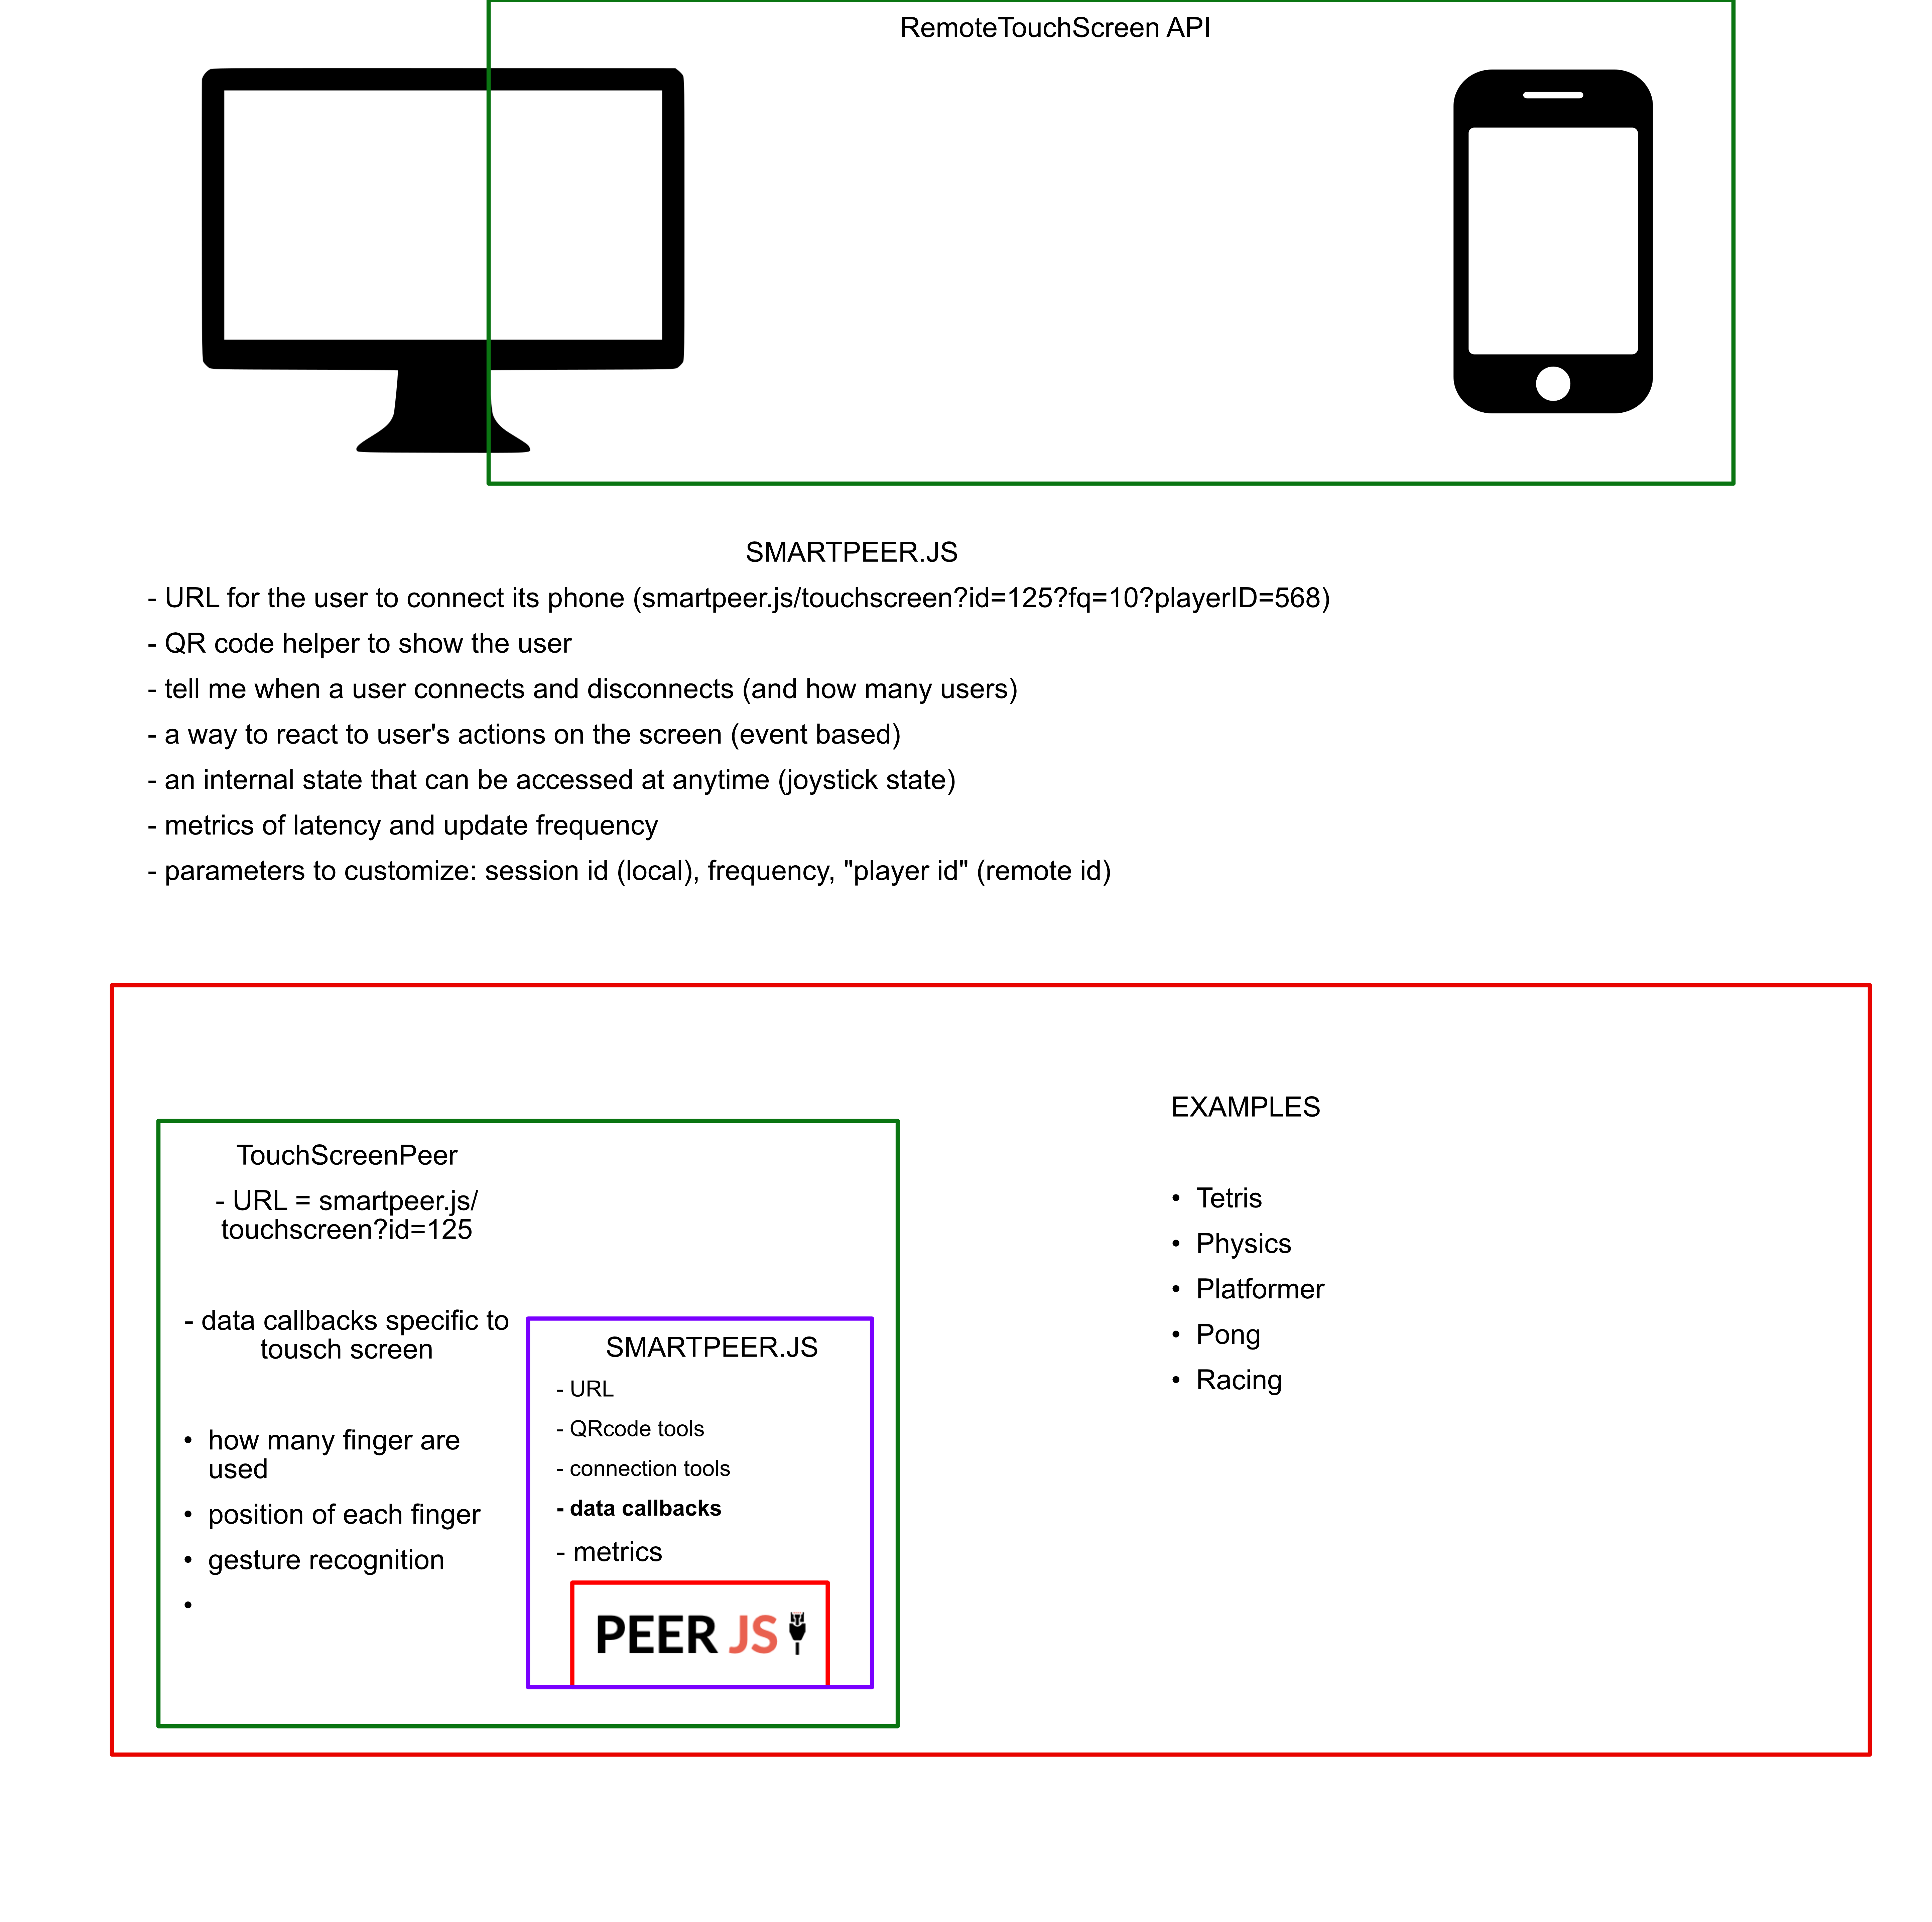
\includegraphics[width=9.7cm]{./images/RemoteTouchScreen.png}
    \caption{Proposed library structure}
    \label{fig:libstruct}
\end{figure}

\subsection{Functional requirements} 
\begin{itemize}
\setlength\itemsep{1em}

  \item \textbf{Automatic handling of the connection :}
  No extra code is needed to create a peer; it is built-in functionality. Both computer and smartphone have their own class to establish the connection.
  
  \item \textbf{Support a large number of players:} 
  Most of the demos from the summer internship were focused on a single player, there is only one that supports two players. The library should have a way of supporting multiplayer functionality by default, it does not impose any maximum number of players the only limitation should be the connection strength. It needs to be simple to keep track of connected players and access the corresponding data from their smartphones. 
  
  \item \textbf{Offer multiple ways of importing the library (import, script tag, download the package):} 
  At the end of the summer internship, it was only possible to use the “import” statement with the library which required further packaging of the code with Webpack. The code should be packaged in a way that offers multiple types of imports to suit different user needs. The package should be available to download via npm, as a min.js file, or use through UNPKG content delivery network. 
  
  \item \textbf{Include statistics calculation, ping, message rate:} The controllers need to be responsive, therefore it should be possible to check the rate of messages being sent from a smartphone as well as ping. This is crucial for building games as the delay needs to be minimal. 

  \item \textbf{Set player IDs:} It should be possible to specify player IDs for each user and not allow any more connections to the same ID. Offer two ways of handling the IDs: keep to the first connection or the last connection.  

  \item \textbf{Host ready to use controllers:} Offer controllers on GitHub pages that are ready to use so that the user does not need to make their own, therefore speeding up the process.
  
  \item \textbf{Make customizable QR codes:} Make a function that will generate a QR code and display it on the screen. The user only needs to specify a DOM element and a controller URL. Optionally, they can set the size of the QR code, player ID, and message throttle. 
  
  \item \textbf{Dedicated classes for different controller types:} In order to keep the code tidy and to make it simple for potential contributors to add their own controllers, there should be a special class for each type of controller with specific fields corresponding to the type of data received from the smartphone. Example: Joystick will have fields to store coordinates and angle while NES controller will store which buttons are pressed. 
  
  \item \textbf{Method to send the controller data from the smartphone:} A dedicated method for sending user type messages that will be identified by the computer as controller data. The user only needs to pass the contents of the message; the labeling is handled by the library.
  

  
  
\end{itemize}
\subsection{Non-functional requirements} 
\setlength\itemsep{1em}
\begin{itemize}
  \item\textbf{ Keep the repository in an organization on GitHub:} In order to appear more professional and to attract more users, the library repository should be kept in GitHub organization. Contributors are more likely to contribute to a project within a dedicated organization rather than a personal repository.
  
  \item \textbf{Create user documentation, demos and, tutorials:} There needs to be clear documentation on the library use, with methods and class explanations. It should be clear how each controller works and how new ones can be made. The documentation should include demos and tutorials on making simple web apps to get the user started quickly and help them understand the library. Each tutorial demonstrates a set of specific features of the library. 
  
  \item \textbf{Publish on npm:} An up-to-date version of the library is published on npm, ready to be installed via the command line. This will make the library easier to find and integrate with other packages used in a given project. 
  
\end{itemize}




%==================================================================================================================================
\chapter{Design}


\section{Working backwards}
Creating an open-source library is a difficult task and there are many details to consider. This is why I chose to use the "working backwards" process. Instead of starting to code the basic functions and classes and then adding methods and features as required, this process focuses on starting with something that would be done at the end. For example, when creating a product for a customer, instead of creating milestones, a time plan, and a set of requirements, the programmers start by writing a press release followed by frequently asked questions, describing user experience, and writing a user manual \cite{back}. Following these steps will make the product building clearer and help design all the features needed. \par
Since my project does not need a press release statement or FAQ page I opted to start with the user documentation. I imagined all of the classes and methods are already programmed. I described what they do, how to use them and included code examples just like any standard documentation. From there, I adapted the current structure and created a time plan based on how important the features and methods in the proposed documentation were. 

\section{Library name survey}
One of the most important things for an open-source library is being found easily. For this reason, I decided to run a survey asking potential users what they would search for if they were looking for this library. The survey was mainly shared on social media pages to get a variety of responses from both, programmers and non-programmers. These include Facebook, Twitter, Discord, Reddit, the P5.js community, and a computing science Ph.D. group. \par
The first task was to look at the existing repository \href{https://github.com/EmmaPoliakova/WebRTCSmartphoneController}{WebRTCSmartphoneController} and try a few demos to get familiar with the functionality. The respondents were then asked to suggest search keywords and a potential name of the library. Most of the keywords featured a combination of words "smartphone", "controller" "game" and "web", for example, web smartphone controller, game controller, rtc smart controller, JS P2P smartphone game. The proposed names were somewhat less suggestive, such as control.io, smart web, remoteJS, Hold It! or ConnectSmartphone. While large companies can afford to name their libraries without indicating what they are used for, a smaller scale project is likely to benefit from a more descriptive name.  \par
I chose to proceed with SmartController which is close to the suggested keywords and descriptive enough to provide a general idea of what the library might be used for. 

\section{GitHub organization}

\begin{wrapfigure}{R}{0.35\textwidth}
\centering
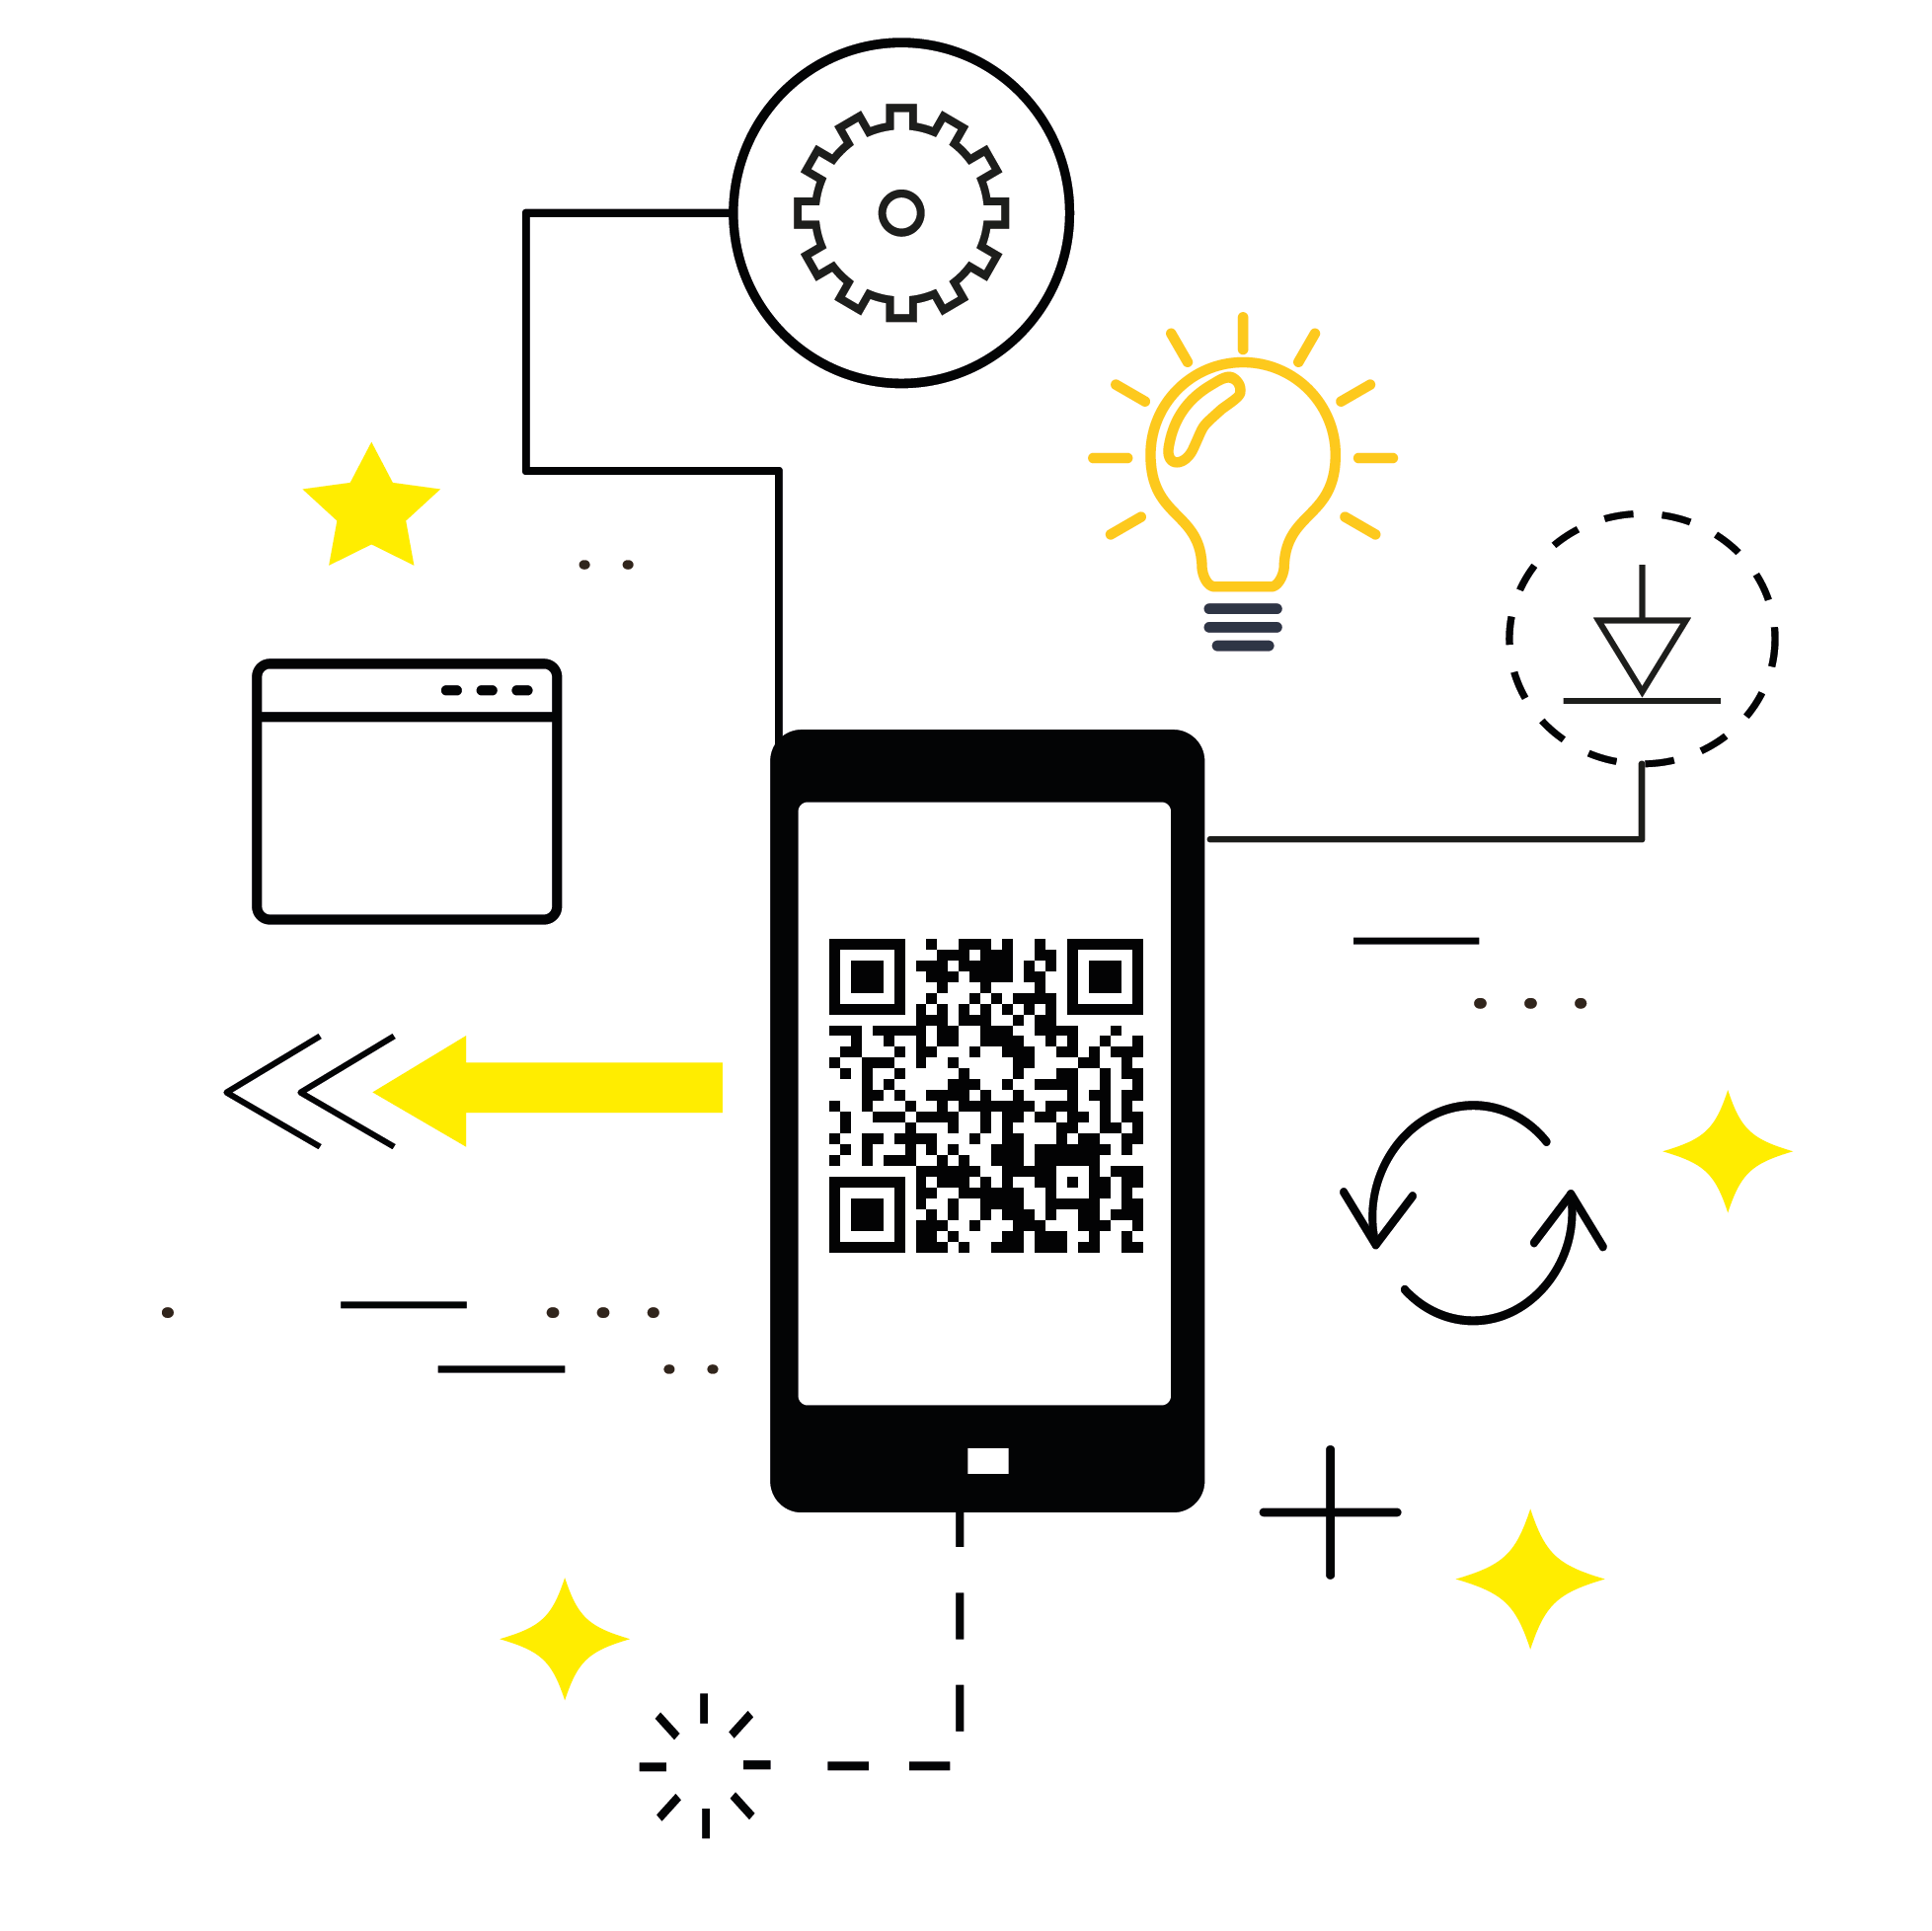
\includegraphics[width=0.35\textwidth]{./images/logo2.png}
\caption{SmartControllerJS logo}
\label{fig:logo}
\end{wrapfigure}

In order to attract users and contributors, I created an organization called \href{https://github.com/SmartControllerJS}{SmartControllerJS} to store all project-related repositories. It includes a repository for the library source code, another repository for the official controllers hosted on GitHub and available to everyone as well as repositories of projects made by other users of the library. The organization has its own logo shown in figure \ref{fig:logo}. It is supposed to symbolize the main features of the library which are a smartphone, a QR code, and a browser. \par

Having a dedicated organization does not influence the quality of code but it will make the library look more appealing and professional than it would be if it was stored on a personal GitHub. On the other hand, a library with a university name could feel too official to potential contributors and this would deter them from creating a pull request to the repository and adding their ideas or fixing bugs. \par 

One of the long-term goals is for the library to grow once the necessary foundations are in place. Whenever a new controller is created, the programmer should have an option to contribute it and expand the library. If a user feels like there is a feature missing or they discover a bug they should have a chance to fix it. All of this is more likely to happen with a professional-looking library that is easy to search for. \par


\section{Library structure}
An overview of the library is shown in figure \ref{fig:libdia}. It offers a quick outline of the library and its classes as well as which components are meant to be used on the computer and which are for use on a smartphone.  \par
The centre of the SmartController library is a class called SmartController. This class is included in the computer side browser and it manages all the connections from smartphones, handles the data input, creates various events such as connection, data, and close. The base of it is a PeerJS object which instantiates a peer ID and a listener for connections. The SmartController class has a list of smartphones peer IDs, and it creates controller objects to store the data of each smartphone. It is also responsible for deleting the list entries when a user disconnects. Finally, it has a method for creating and displaying QR codes.\par

\begin{figure}[h!]
    \centering
    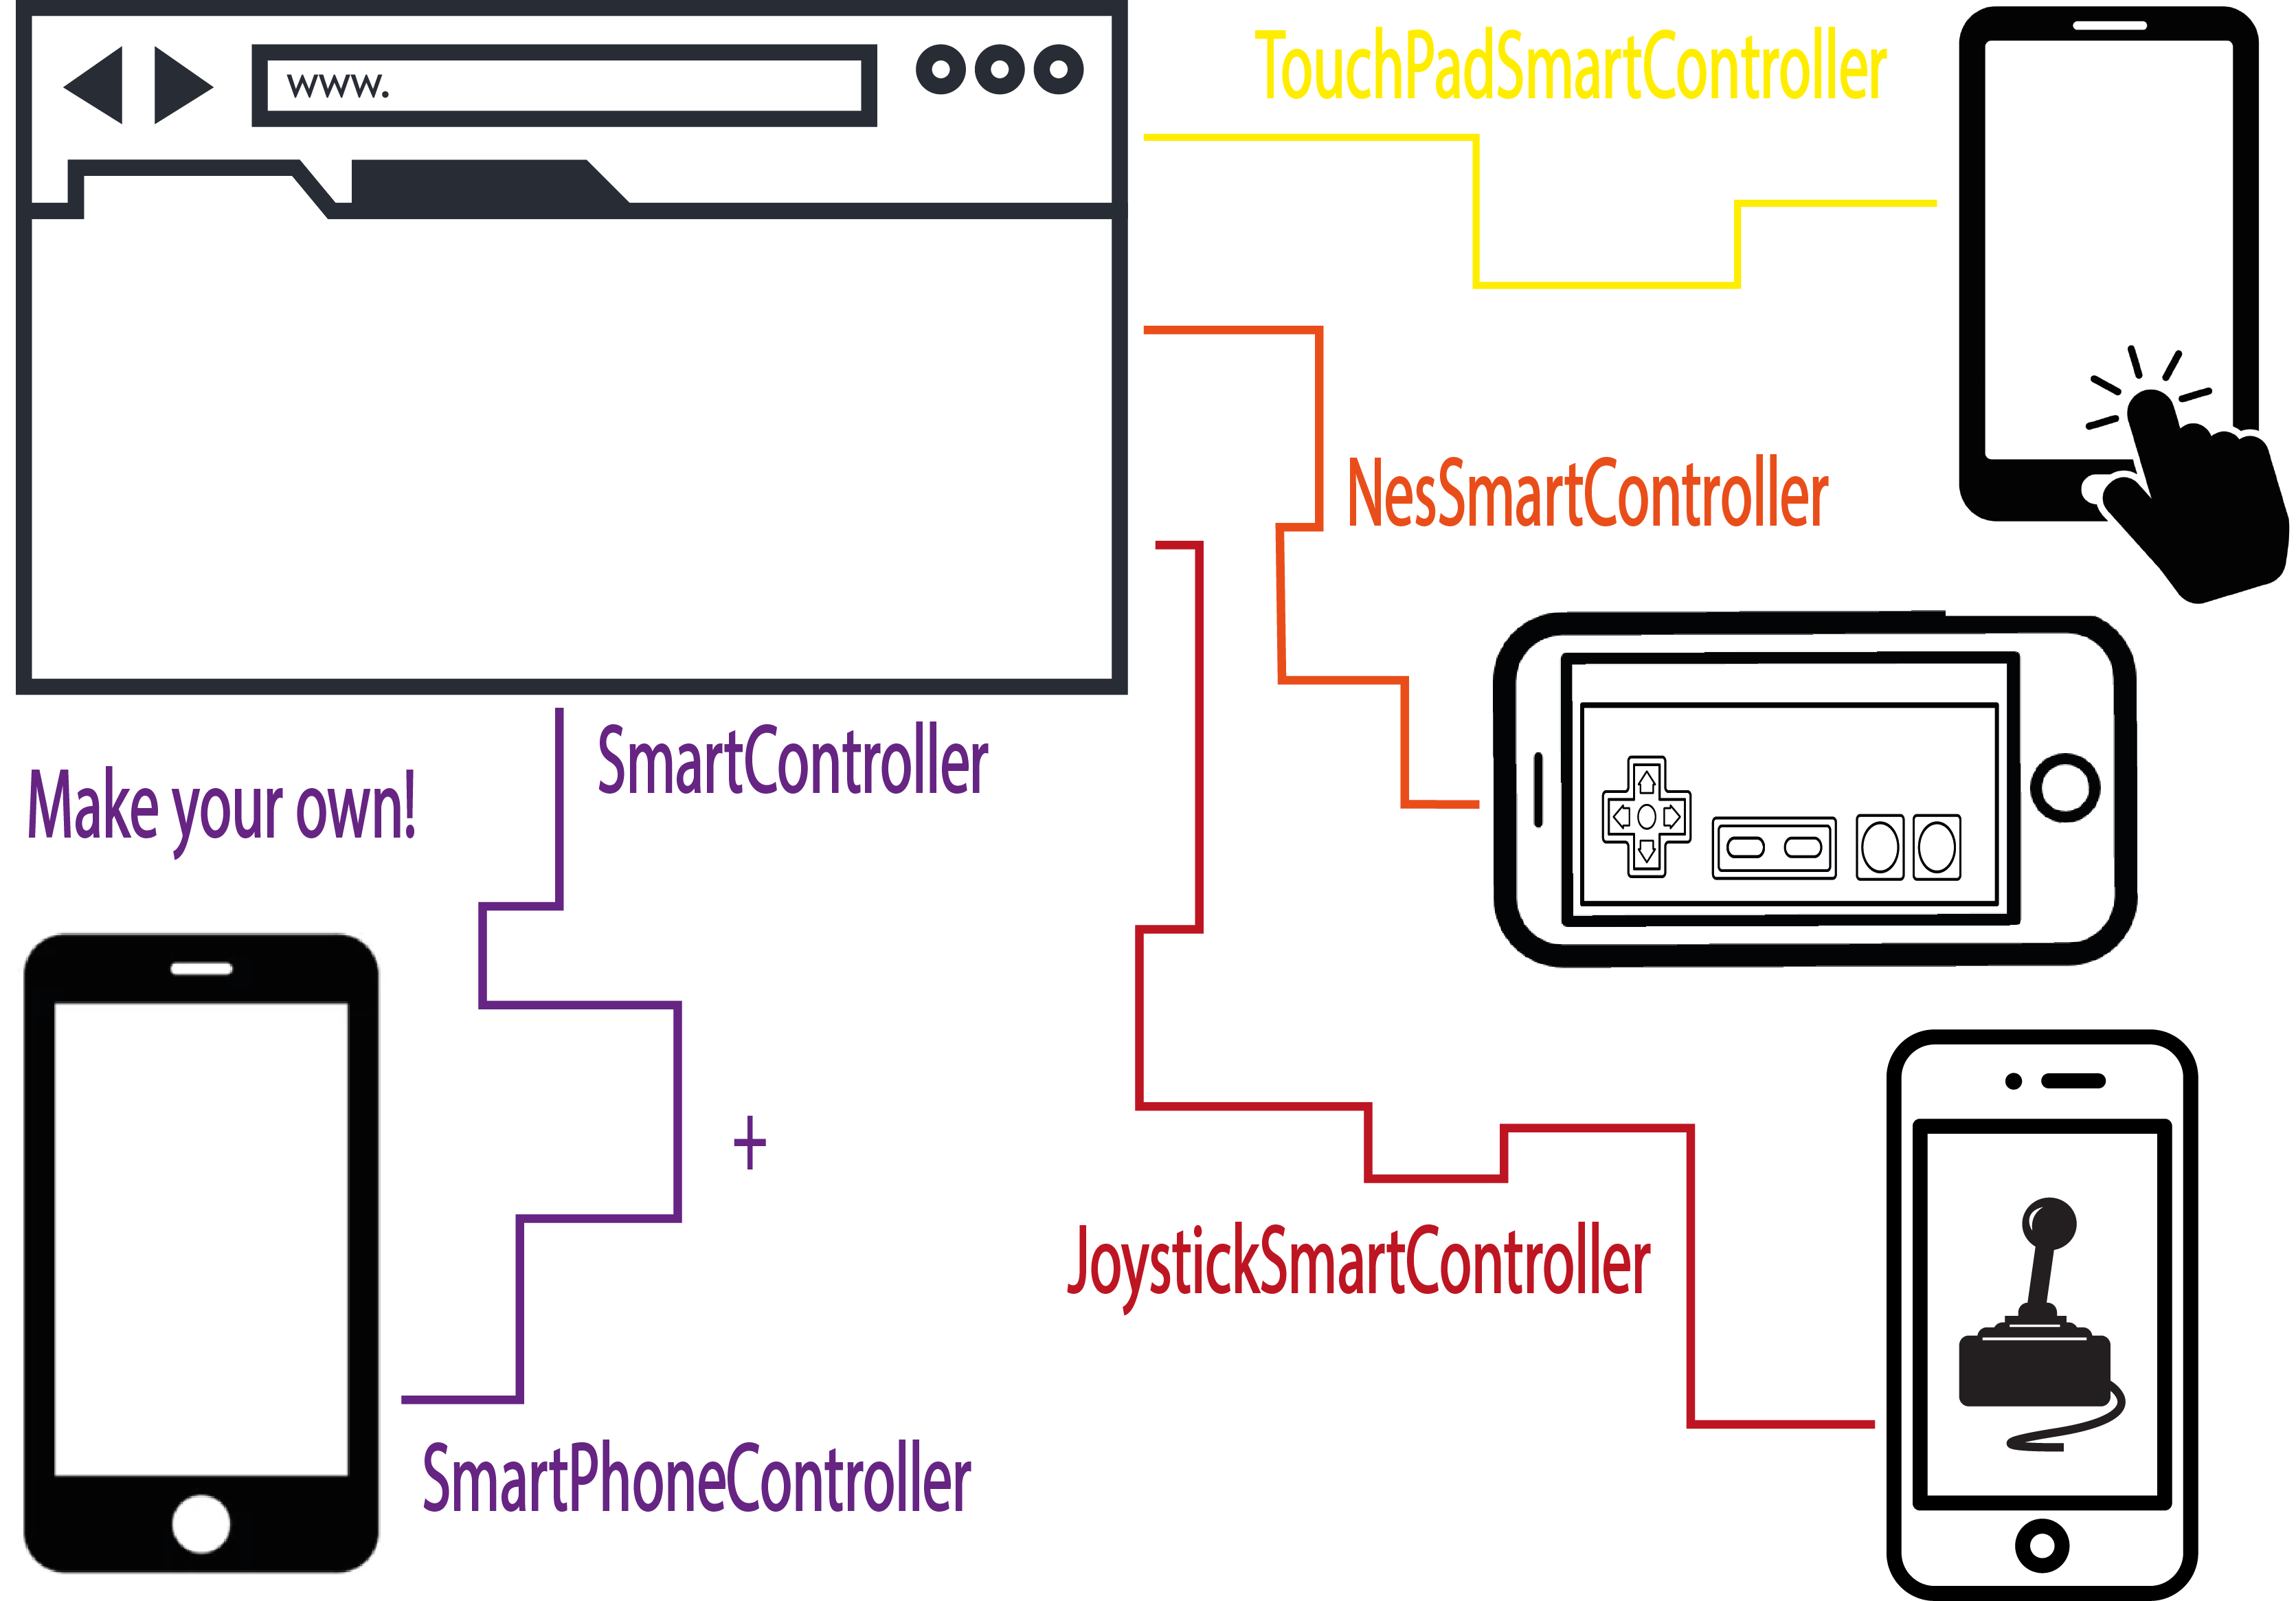
\includegraphics[width = 10cm]{./images/All.png}
    \caption{Library structure diagram}
    \label{fig:libdia}
\end{figure}

\pagebreak
Every time a user connects a new BaseController object is created. This class is responsible for storing a peer ID and displaying the data from smartphones. Although not shown in figure \ref{fig:libdia}, it is a building block for every more complex controller object. On its own, it simply takes the smartphone data and prints it in the console. It offers a method to be overwritten to process the data in a specific way a user desires. It is also important for keeping the structure of the library and any new controller created clear. \par

TouchPadSmartController, NesSmartController and JoystickSmartController extend SmartController. These classes match specific type of smartphone controller and will trigger a creation of matching controller objects in the SmartController class. They do not offer any extra functionality apart from passing a different controller class to SmartController, a one that replaces BaseController. This once again helps to maintain a specific structure and anytime a new controller class is created no changes need to be made directly in SmartController class. \par 

The class that handles the connection in the smartphone browser is SmartPhoneController. It is designed to read parameters from a URL and connects to the computer browser. It is important to note that since SmartPhoneController accesses the parameters automatically, the URL needs to follow a specific format in order to create the connection. It then stores a player ID if it was specified, sets an optional message throttle, and lets a user send the controller input to the computer. \par

The overall structure allows for the easy addition of any new features and methods. While figure \ref{fig:libdia} is a final layout for this project, it is likely to change in the future as the library continues to evolve and improve.


\section{Technologies}

\subsection{JavaScript}
The SmartController library is written entirely in JavaScript. JS is a high-level programming language with dynamic typing. It is one of the core programming languages used for the creation of web pages along with HTML and CSS. All major browsers have an engine dedicated to executing JavaScript code. \cite{js} \par 
The two main reasons for choosing JavaScript to make this project are that the library is centered around creating interactive web applications and controllers which are also essentially websites. The other reason is that the necessary package PeerJS also uses this language.  

\subsection{PeerJS} 
PeerJS wraps the browser's WebRTC implementation to provide a complete, configurable, and easy-to-use peer-to-peer connection API. \cite{peerjs}. It simplifies the use of WebRTC through the distribution of peer IDs via a broker server to establish the peer-to-peer connection between two browsers and start a data stream. It can handle both, generic data as well as audio and video calls. PeerJS is at the centre of the SmartController library and makes communication between the smartphone and the computer possible. \par
PeerJS also provided a great deal of inspiration in terms of structuring the repository and packaging the module. 



\subsection{EventEmitter2}
Smartcontroller uses many different events to inform the user about the connection and data. The event triggers and listeners are created with EventEmitter2. An event emitter is a pattern that listens to a named event, fires a call-back, then emits that event with a value. \cite{event}. It can also be referred to as the “pub/sub” model. The programmer must have a way of reacting to important events such as opened or closed connection, or the incoming data. EventEmitter2 is an ideal choice as it has better performance and is browser compatible compared to the standard EventEmitter module. \cite{event2}.

\subsection{Parcel}
Parcel is a module bundler. It takes all used modules and their dependencies in a project and bundles them into a single file. This project requires a bundler as it relies on other npm modules. Unlike Webpack, there is no configuration for Parcel and the bundling process is very fast. Bundling the SmartController into a single file offers multiple ways to import it into a project.

\subsection{EasyQRcodeJS, NippleJS, Plotly}
Other libraries used in this project are EasyQRcodeJS, NippleJS and Plotly. \par 
The QR codes are generated with EasyQRcodeJS. This library offered many useful settings for the QR code and also supports customization with pictures and colours and thus giving an option to personalize every aspect of the website a programmer is creating.  \par
NippleJS is a joystick library. Compared to other JavaScript joysticks, it can produce many different types of information about the position, angle, and force used. This was an ideal library to use as it gives the user freedom to choose which of the provided information they want to use and they do not need to rely solely on xy coordinates. \par
Plotly is a plotting library for JavaScript. It is used on the statistics evaluation page. It has many convenient plotting features, it is easy to use and the graphs displayed on the page can be saved in png format.


%==================================================================================================================================
\chapter{Implementation}
The library offers a range of tools for creating interactive websites and new controllers. This chapter describes the implementation of the individual features, how to access and install the module, documentation of the code, and known limitations.

\section{Features}

\subsection{SmartController}
SmartController is the main building block of the library. SmartController object needs to be created in the computer browser to allow for new connections and their management. It is possible to specify the peer ID itself, how to handle new connections and whether the statistics should be calculated. The constructor takes optional peer ID, firstConnected Boolean value, stats Boolean and, a controller class. It then creates a new PeerJS object which will either use the provided ID or generate a random one for other peers to connect to. Figure \ref{fig:flow} illustrates simplified inner logic of SmartController class.\par 

\begin{figure}[h!]
    \centering
    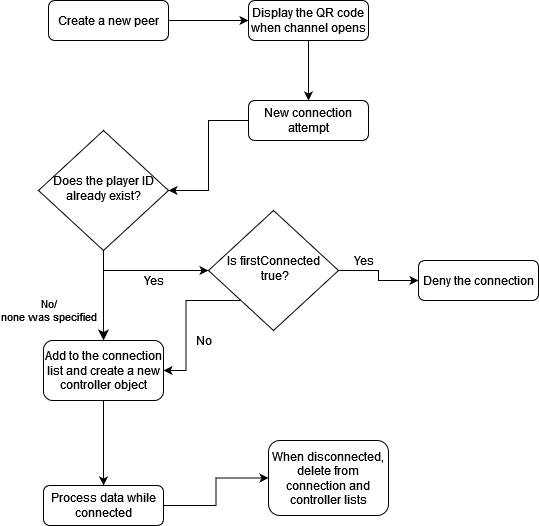
\includegraphics[width = 10cm]{./images/statediagram.png}
    \caption{Simplified SmartController flowchart}
    \label{fig:flow}
\end{figure}

\subsubsection{QR code method}
Once the channel is open for connections, a QR code method can be called to generate and display a QR code. The user can use this method to modify the behaviour of the controllers that will connect through the code. It is possible to specify the player ID and message throttle in milliseconds. The size of the QR code is customizable. It has a list of currently connected controller objects and smartphone peer IDs. It has only two non-optional parameters, an HTML div element needs to be provided for the QR code to be generated and a URL of the controller. All of the arguments are combined in a single link which is used to create the QR code. \par 

\subsubsection{Handling new connections}
After a QR code is displayed and a new connection between a smartphone and a computer is established, the SmartController will store this connection in a list, then generate and store a new controller object. The parameter firstConnected specified when creating a SmartController object helps to handle connection management. If no player IDs are specified for smartphones, then all connections are stored and used. If there is a player ID specified and firstConnected is true, SmartController will check if an ID is already stored in the connection list. If yes, no further connections to that ID will be allowed. If firstConnected is set to false, every new connection to the same player ID will overwrite the original one. \par

\subsubsection{BaseController} 
After a smartphone peer has been successfully added to the connection list, SmartController generates a BaseController object. This object will be responsible for processing the data for an individual smartphone. This is the most basic, default version of a controller object therefore it only stores a peer ID, a player ID if it has been specified and, statistic fields for ping and message rate. The updateController method does not process the data in any way, it simply logs them in the console. 

\subsubsection{Events} 
When the connection procedure is complete, the smartphone is ready to be used for controlling the website. The user can choose if they use state actions, that is the data stored in the controller object at all times or if they create listeners for different events offered in the SmartController. The available events are \emph{connection}, \emph{data} and \emph{close}. Connection means that the user will be notified upon a new connection along with the peer or player ID. Data signals the incoming data produced by the smartphone controller, the event passes the ID of the smartphone that sent this message along with the contents. Finally, close will alert the user of a particular smartphone controller disconnecting. When a smartphone has disconnected, the peer ID and the player ID are removed from the connection list and the controller object is destroyed.  \par 

\subsubsection{Statistics}
The final feature SmartController provides is statistics calculation. Just like firstConnected, the stats argument can be set to true and false. It is true by default. This means that once a connection is established, the computer and the browser will keep exchanging empty messages to calculate ping and the number of these messages sent per second. The times are stored in a list that is part of BaseController. The list is periodically checked and all messages older than one second are deleted. 


\subsection{TouchPadSmartController, JoystickSmartController, NesSmartController}
These classes extend SmartController. The only difference to SmartController is that they replace the BaseController with a different class. All of the controller classes extend BaseController but have a different way of processing the data and offer extra fields to store specific information. \par

\subsubsection{TouchPad class} TouchPad class adds isActive state which is true when the player is interacting with the phone screen and false otherwise. It has a state field which stores xy coordinate pairs for each finger touching the screen and finger\_number field for the number of fingers used. 

\subsubsection{NesController class} NesController extends the BaseController with buttons dictionary. Initially, each button value is set to false. When a button is pressed on the smartphone its value in the dictionary changes to true. It will switch back to false once the button is released. 

\subsubsection{Joystick class} Joystick class adds isActive field which works the same way as in TouchPad. It also has a state field that stores information on the angle, direction, distance, position coordinates of the joystick. The updateController method in the class calculates by how much the position changed from a previous state from the new angle. This can be useful if the user is trying to move an object on the screen. In that case, they simply need to add the positionChange values to the xy coordinates of the object.

 
\subsection{SmartPhoneController}
SmartPhoneController sets up the peer and connection on the smartphone browser side. The connecting to the computer is fully automated and handled upon the SmartPhoneController object creation. It reads the parameters from the URL, an example of the URL structure can be seen in figure \ref{fig:url}. First, it will find out which peer ID is the smartphone meant to connect to. Then it checks if a player ID was specified. After that, it sets the message throttle. The URL needs to follow a specific format otherwise the connection process will fail. \par

\begin{figure}[h!]
    \centering
    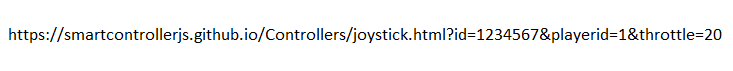
\includegraphics[width = \textwidth]{./images/url.png}
    \caption{Example of controller URL}
    \label{fig:url}
\end{figure}

After all the parameters have been saved and the connection is open the smartphone sends a setup message with its screen dimensions. If the statistics messages are allowed, the exchange of these also begins at this point. The user can use the method sendMessage to send any data produced by the controller to the computer. The method labels the data as user type so it can be distinguished from statistics messages and passed to the controller object for further processing. Overall, the creation of a controller is very simple and requires only a couple of lines.

\subsubsection{Message Throttle} It is possible to set a message throttle that will control how often user messages are sent. The interval is set in milliseconds. For example, in figure \ref{fig:url} the throttle is 20ms. This means that a message will be sent every 20ms and the rest will be discarded. When the controller tries to send a message, it is checked against the last time a message has been sent. If it is less than 20ms then the message is discarded otherwise it is sent to the computer and the last message time is updated. The message throttle is not suitable for all controllers, especially those who track the activity status. It could happen that a button was released but the message got ignored so the button will show as active to the computer browser.\par 

\subsection{Hosted controllers}
There is a variety of controllers hosted on GitHub pages to help the user to get started quickly if they opt to use an already created controller. Currently, there are NES controller \ref{fig:nes}, joystick \ref{fig:joystick}, touchpad and a prototype of a basic accelerometer.  The controllers are kept in a separate \href{https://github.com/SmartControllerJS/Controllers}{repository} from the \href{https://github.com/SmartControllerJS/SmartController}{SmartController} library. In addition to the controllers the repository stores tutorials and the statistic page. All URLs are available in the accompanying README.md file. To use any of the controllers, the user simply needs to pass the controller URL to the QR code method. \par 
The controllers are bundled with Webpack locally and the built version is published on GitHub pages to be used. They offer a broad range of data and buttons. This is because they are not specifically tailored for a single application and the library is trying to achieve broad coverage of use cases. 

\begin{figure}[h!]
    \centering
    \begin{minipage}{0.45\textwidth}
        \centering
        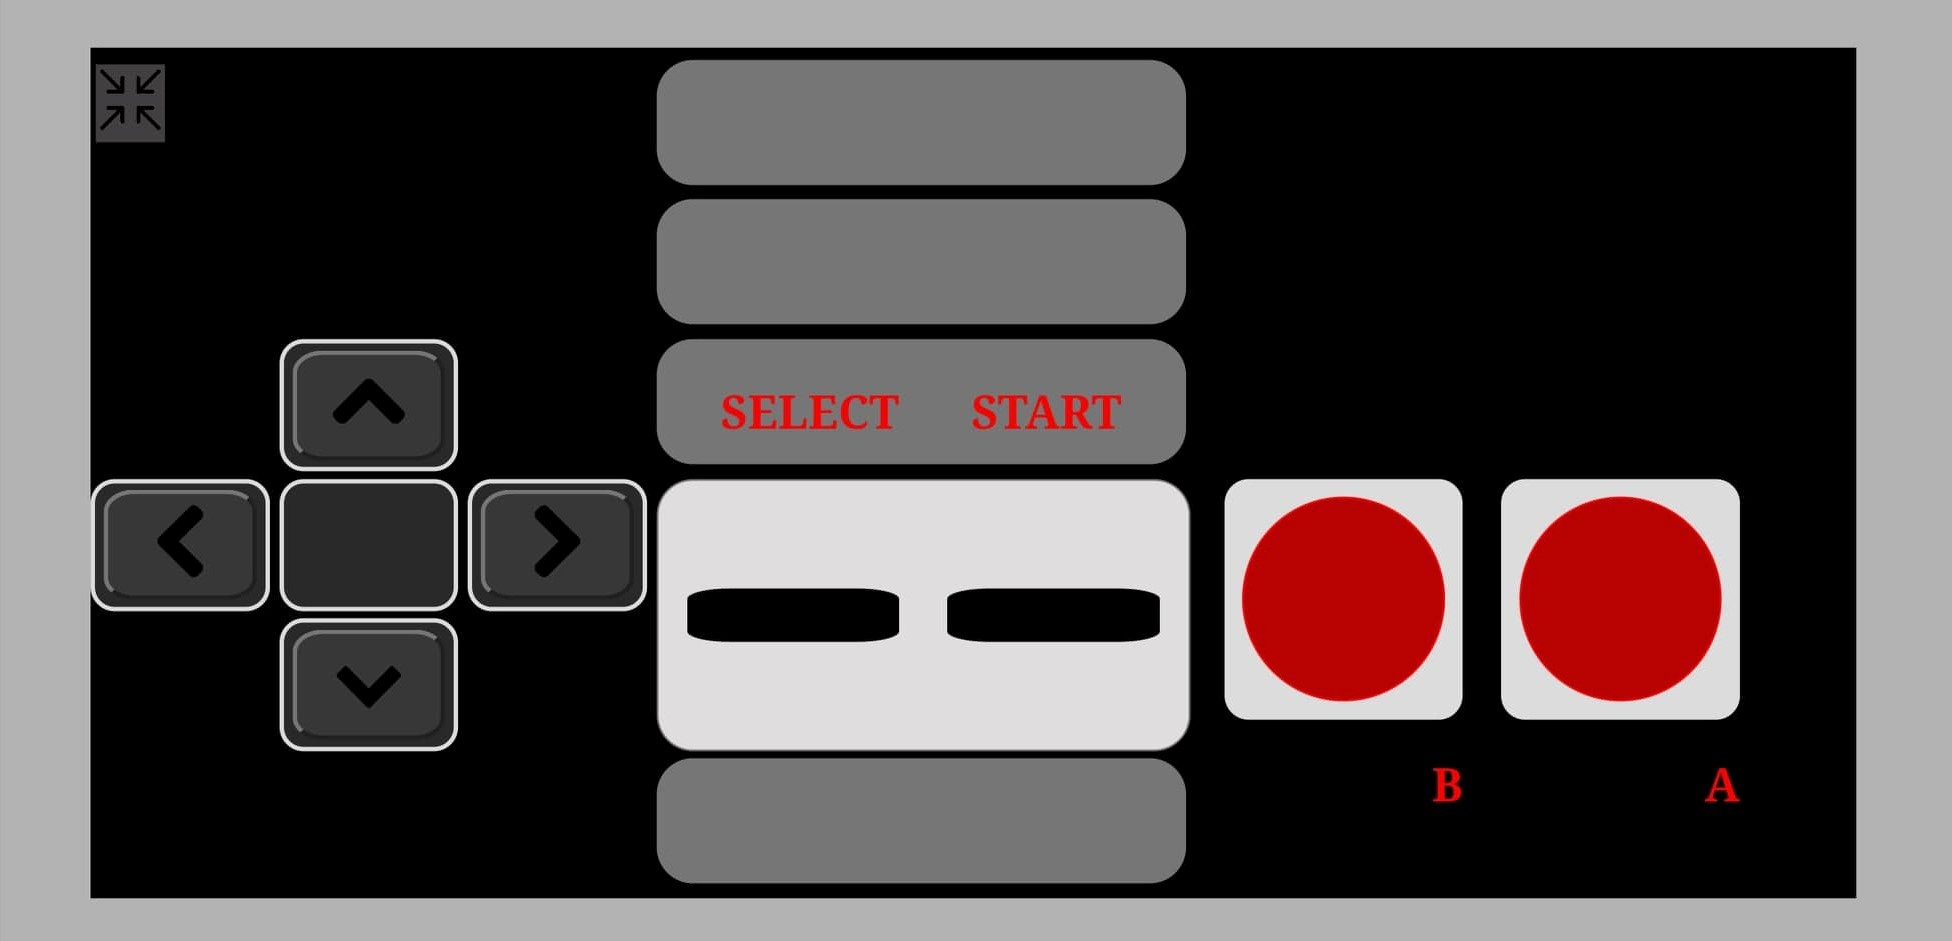
\includegraphics[height=4cm]{./images/nes.jpg} % first figure itself
        \caption{NES controller}
        \label{fig:nes}
    \end{minipage}\hfill
    \begin{minipage}{0.45\textwidth}
        \centering
        
\includegraphics[height=4cm]{./images/joystick.jpg} % second figure itself
        \caption{Joystick}
        \label{fig:joystick}
    \end{minipage}
\end{figure} 

\section{Deployment}
The library is bundled with Parcel into a file called smartcontroller.min.js. It is then published to \href{https://www.npmjs.com/package/smartcontroller}{npm}. This gives the users several options of including it in their project. It can be installed via npm, shown in figure \ref{fig:npm} and used with import statement in combination with bundlers such as Webpack or Parcel. It can be added to the Html file via script tag with \href{https://unpkg.com/}{unpkg} link as in figure \ref{fig:unpkg} and the minified file can also be downloaded and added to the project folder directly. 

\begin{figure}[h!]
    \centering
    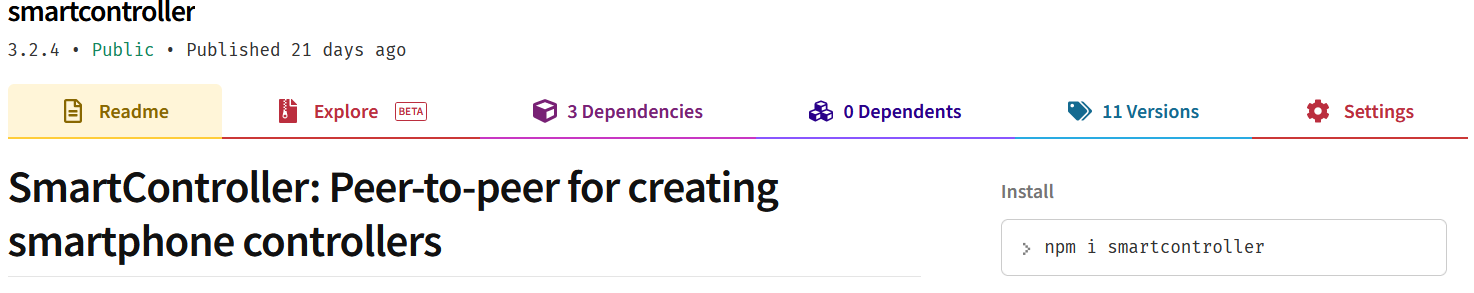
\includegraphics[width = 10cm]{./images/npm.png}
    \caption{Npm website}
    \label{fig:npm}
\end{figure}

\begin{figure}[h!]
    \centering
    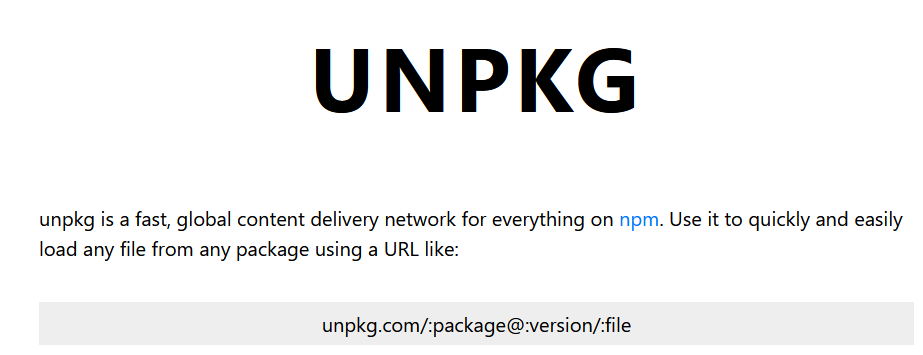
\includegraphics[width = 10cm]{./images/unpkg.png}
    \caption{UNPKG website}
    \label{fig:unpkg}
\end{figure}

\section{Documentation}
The \href{https://smartcontrollerjs.github.io/SmartController/}{documentation} page is made with Jekyll and deployed via Github pages. It includes a basic description of the library and a getting started page. \par
The introduction page has a diagram \ref{fig:libdia} that shows how the classes are connected. It also showcases demos made during the summer internship to help demonstrate what is possible to make with the library. This helps the user to familiarise themselves with the usage. \par
The getting started page presents how to import the library and create a basic SmartController object to manage the connections in the browser. It shows the user how to generate a QR code and listen for connection and data events.\par
There is a detailed description of all available methods and events provided in the SmartController class. Each controller has its own page describing the type of data that is stored and how to access it. The SmartPhoneController page describes how to build a web page for a smartphone and how to send the messages to the computer browser.\\

\begin{figure}[h!]
    \centering
    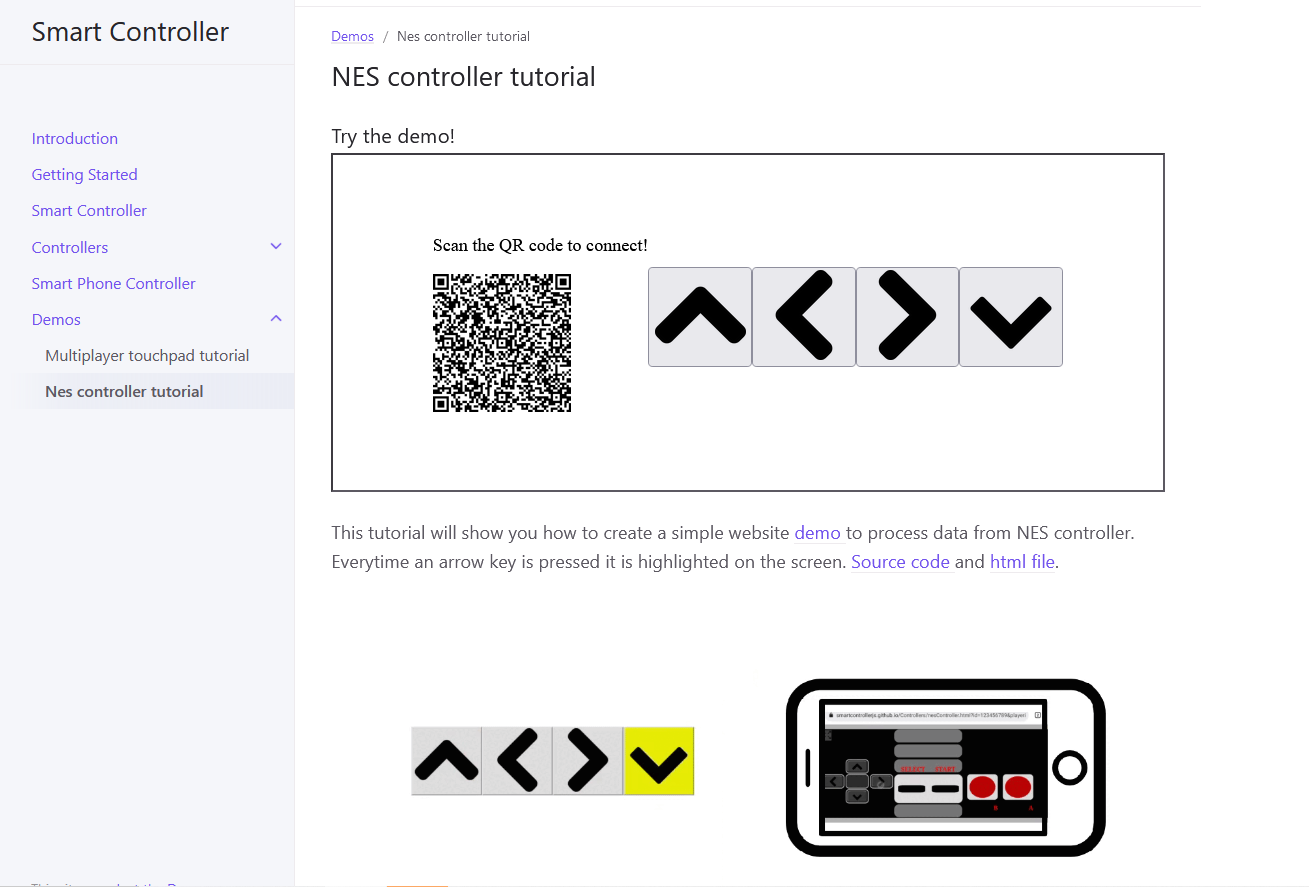
\includegraphics[width= 10cm]{./images/document.png}
    \caption{Documentation page with embedded demo}
    \label{fig:demo}
\end{figure}

Finally, there are detailed tutorials that will guide the user to create their own projects. The first demo shows how to handle a single-player input from the NES controller. The second demo teaches the user how to create a simple multiplayer game. 
Figure \ref{fig:demo} shows a demo embedded directly in the page so the user can try it out without having to open a new tab. A more detailed version of each demo is available on a full page, including steps to follow to allow the user to try out different features of the library.

\section{Signaling server}
PeerJS offers a signaling server to distribute the peer IDs by default. When creating a new peer object, it is possible to specify a custom server instead. Following the official server outage, I opted to deploy my own instance of peer server to Heroku. This was a simple process as PeerJS has a pre-packaged code that is ready to be deployed without extra settings. I then replaced the default server with my own domain. The advantage is that there is a smaller probability of peer ID clashes, there are many more users on the official server compared to a private one. The disadvantage is that I am responsible for maintaining the server instead of PeerJS. The loading of the QR code got slightly slower in some demo instances as well.

\section{Limitations}
During the development, I have encountered several limitations that can be addressed with varying results. The most complicated issue to solve is broad bands specific security settings that prevent WebRTC from sending messages between peers or block the connection altogether. The connection can fail to be established, this means that the broad band blocks the use of the PeerJS library. The other case is when the connection is created but no messages are sent. This is most likely a result of a specific port being blocked and therefore the messages cannot get through. It is difficult to fully control this, however, a proposed solution is to set a time out on receiving the initial setup message. If it does not arrive within a set time frame, the user should be informed that it is not possible to start the communication between the two browsers. \par 

The other main issue encountered applies to selected browsers that do not support or block WebRTC. These were found to be Brave Browser and Safari. Once again, this problem is difficult to solve fully but a similar approach with a timeout message could be adapted. It might also be possible to track which browsers are causing issues for the library by creating a server that would be informed when a timeout happens. The data could then be included in the documentation to help the user to develop their web application. This solution was not possible to implement during the time frame of the project. \par

The last issue is related to selecting specific peer IDs. The user is allowed to specify their own peer ID, however, this means they need to be aware of potential clashes as there cannot be two peers with the same ID. That is opening the website with static ID twice would result in only one of them working. The users are informed about this in the documentation and it is recommended to use a specific ID only during the development stages.




%==================================================================================================================================
\chapter{Evaluation} 
This section includes a user interview and analysis of two different use cases: all players playing locally via the same connection and one player playing locally with the rest of the players viewing and controlling the game through screen sharing. The user interview consists of 6 questions and is focused on evaluating the experience and improvement of any future development. There is a performance comparison between different controllers. The evaluation uses three Android devices to measure the performance of each one of them. Finally, the chapter looks at how the message throttle parameter influences the user message rate. \par 
The statistics section shows graphs for joystick and touchpad only. NES controller was also tested for ping and message rates. The results were very similar to the other two controllers and the remaining graphs can be found in the appendix.

\section {Working with users}
During the project, I got to work with two fellow students. They were using it for their project. It was a very valuable experience for developing the SmartController. They were the first users and provided great input on both the functions available and the documentation. I have become very familiar with the project after working on it during my summer internship and also for two semesters in year 4. Therefore, it can be difficult to distinguish what should be included in the documentation and what is redundant. Through explaining how my library works I learned which things needed to be demonstrated more clearly and what examples of code would help the users to understand how to use the library. \par
The students used the library in combination with various game engines for their own projects and this became an important source of information on integration and errors. With the amount of devices, browser game engines, and game mechanics, it is impossible for a single person to test every use case for errors, therefore, discussions with users during the development of the library helped to prevent and fix early problems. \par 
At the end of the project, I conducted a short formal interview with both of the students to evaluate the overall experience they had and to discover any weaknesses and shortcomings. Below is the analysis of responses to each question as well as proposed solutions for every mentioned issue: 

\textbf{Q: Is there anything you found good about using the library?} \\
Both students agreed that overall, the library was easy to use and the demos in the documentation were very helpful and demonstrated the use cases well. The amount of documentation was likewise praised. The conclusion for both participants was that they did not have much difficulty using the library for their projects. \par

\textbf{Q: Did you have any issues using the library? If yes, what were they?} \\
The issues were mostly related to the novelty of the library, not being familiar with the workflow. The main issues mentioned were ID clash and having to manually update the library version number in the import URL. The peer ID clash caused confusion because two peers cannot have the same ID therefore when there were multiple copies of the website opened at the same time only one of them would show the QR code. This problem has been addressed both in the documentation and with a warning message if the QR code is not showing. \\
Currently, the demos use a URL that has a specific version of the library included. It would be useful to upgrade the documentation with a link that automatically uses the latest version when the import is happening via UNPKG. \par

\textbf{Q: Did you find the documentation useful?} \\
The documentation received very positive reviews. The demos were appreciated by both students. Other positive elements mentioned were good coverage of the use cases, getting started page allowed a quick start. To summarise, the students agreed that the documentation pages provided a good reference point for the library. \par 

\textbf{Q: Is there anything that was missing in the documentation that would have helped you to understand the library better?} \\
The critique was mostly focused on the initial version of the documentation that had no demos. It has since been updated and reworked completely, including demos and tutorials. Other than that, it was mentioned that it would be good to have a more detailed explanation of each controller, as they store different types of data and are structured differently and this can be a source of confusion. \par 

\textbf{Q: Do you think your project would have benefited from a custom controller? If yes, why did you opt for a pre-made controller?} \\
Both students stated that a custom controller would have improved their projects. The primary criticism was that the available controllers offer more functionality than they needed, for example too many buttons or too much information was being sent that was irrelevant to the projects. There were also elements missing that could have been useful, i.e. a controller that has both buttons and a joystick would suit the project more than buttons only, of which most are not being used. \\
The reason for not making a new controller was the lack of time in both cases. The available controllers were not a perfect fit but they worked well enough to not be included on the priority list.  \par

\textbf{Q: Would the tutorial on SmartPhoneController help you make your own controller?} \\
For the last part of the interview, the students were asked to look at the \href{https://smartcontrollerjs.github.io/SmartController/smartphonecontroller.html}{SmartPhoneController} page. It briefly describes how to use the SmartPhoneController class and how to make a simple accelerometer. The tutorial was deemed useful but there were some suggestions made on how to improve the page. It could be by showing tutorials for both browsers side by side. The reason for this is that the user could see how the newly made controller can be processed on the computer once the message is sent. The other suggestion was on showing more elements for controller building, for example, buttons or joystick, and possibly breaking down the already existing controllers into tutorials. \par

\section{Statistics}
There is a range of different statistics available to the user to monitor the performance of the library. These can be switched on and off as needed. If the f statistics parameter is switched off then ping and the statistics message rate are not available. Figure \ref{fig:statspage} shows a dedicated web page for measuring ping, user message rate, and statistics message rate. The user can input a URL to their own controller or use one of the available ones to measure performance in different areas. The webpage can export the data from the evaluation to CSV. The graphs are created with Plotly library. It offers many convenient plotting functions one of which is the ability to directly download the created graphs. \par 
The measurements that include remote devices were made through screen share. The statistics page was displayed on a Teams call and the participants were asked to scan the QR codes with their smartphones. The simulation ran for around 500 frames each time. 

\begin{figure}[h!]
    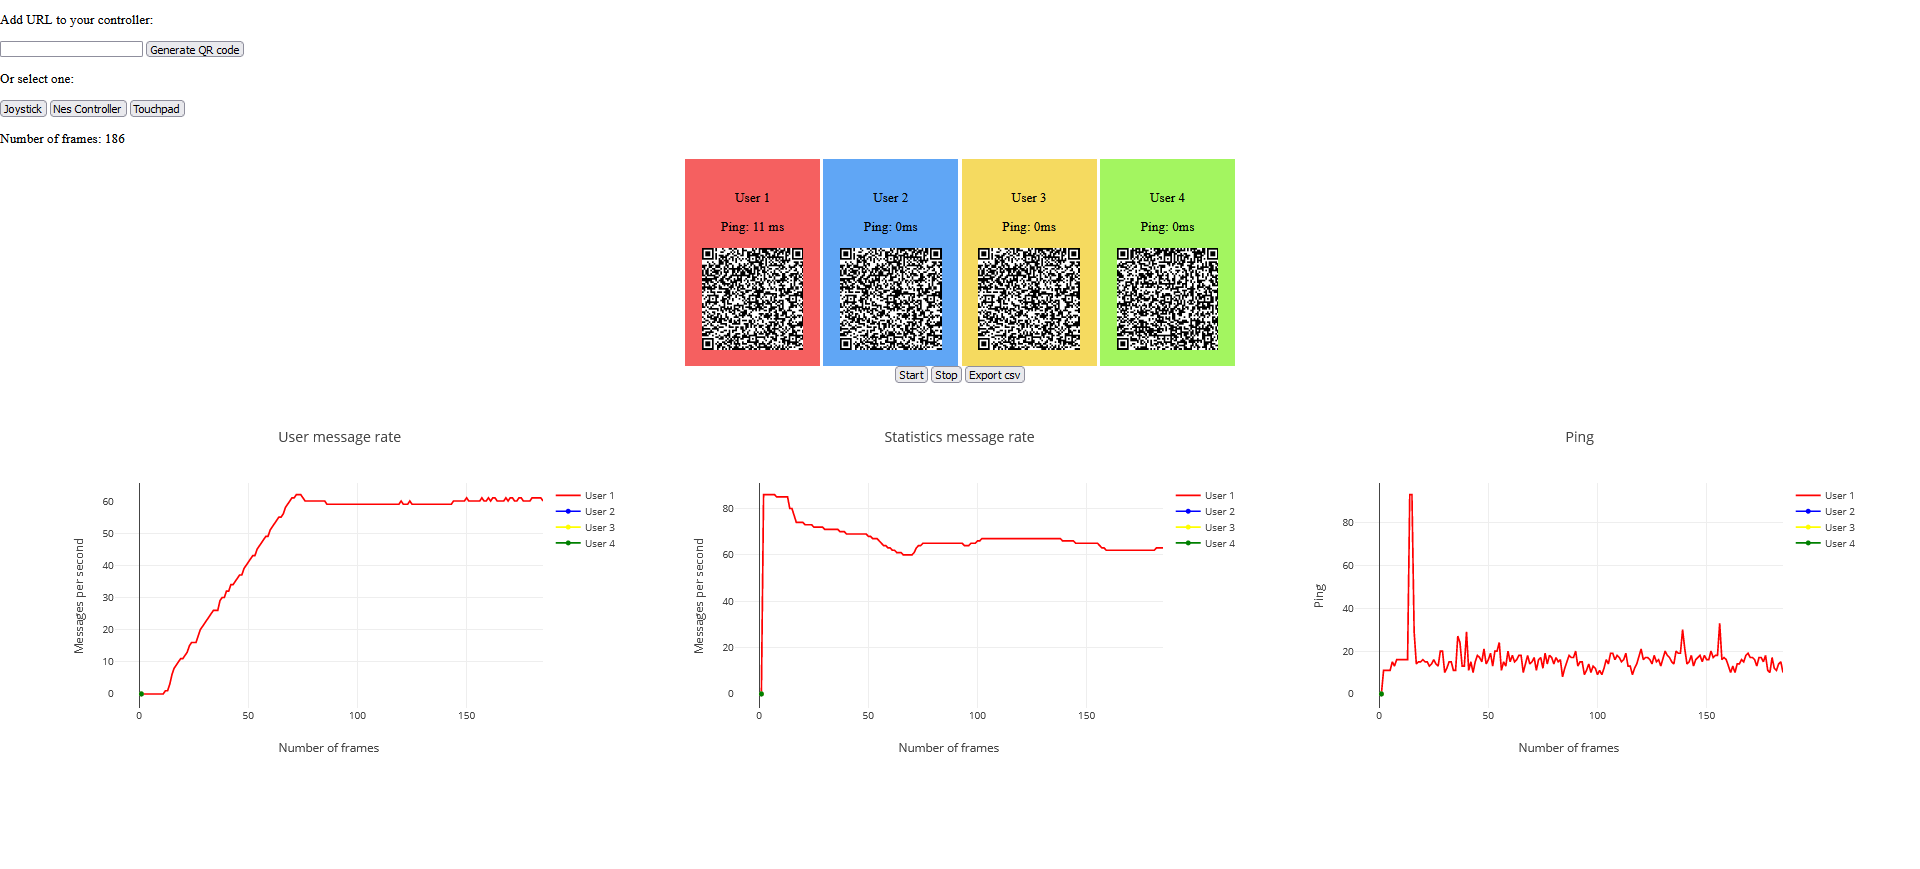
\includegraphics[width=\textwidth]{./images/statspage.png}
    \caption{Example of measurements created with the statistics page}
    \label{fig:statspage}
\end{figure}

\subsection{Ping}
The first statistic in question was ping. Each controller has a ping field. It is calculated in milliseconds as a round trip between a computer and a smartphone. Low values of ping are preferable to higher ones, especially when gaming. When ping is high, there is a delay to the actions made by the player, so-called lag. For example, they tell the character to move but with high ping, it might take a few seconds for the required action to happen. This is very frustrating in general, even more so when the game requires great accuracy \cite{latency}. Great ping value for gaming is around 20ms and values between 40-100ms are still considered very good \cite{ping_value}. \par
Figures \ref{rjoyping} and \ref{rtouchping} show the ping of one local device and two remote devices. There is a clear separation between the red local smartphone and the blue and yellow remote phones. Using the device locally resulted in ping around 20ms while the remote devices oscillate between 40ms and 80ms in the case of the joystick and 40ms - 60ms for the touchpad. This demonstrates that even with the controllers connected to a different network than the computer browser it is still possible to achieve a very good experience with little lag.  \par
\begin{figure}[h!]
    \centering
    \begin{minipage}{0.45\textwidth}
        \centering
        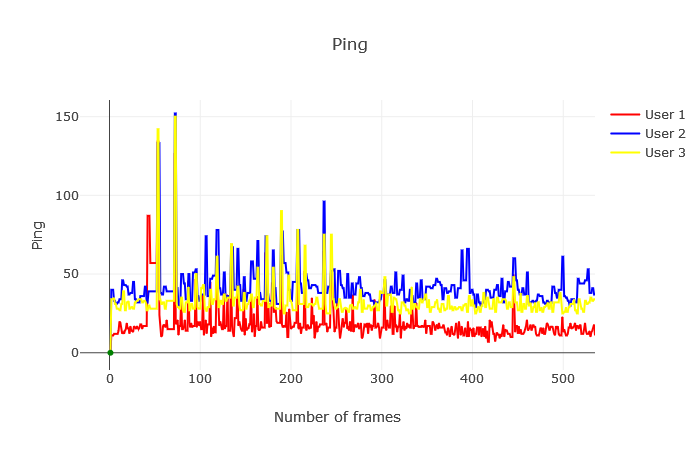
\includegraphics[width=7cm]{./images/rjoyping.png} % first figure itself
        \caption{Remote joystick}
        \label{rjoyping}
    \end{minipage}\hfill
    \begin{minipage}{0.45\textwidth}
        \centering
        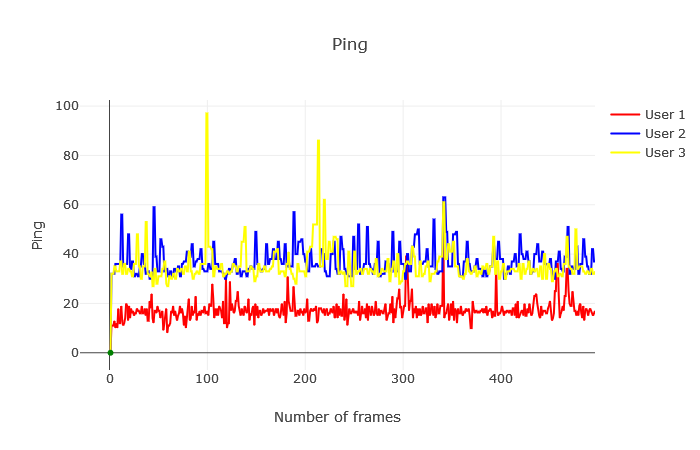
\includegraphics[width=7cm]{./images/rtouchping.png} % second figure itself
        \caption{Remote touchpad}
        \label{rtouchping}
    \end{minipage}
\end{figure}

There are occasional ping spikes when the ping values double or triple and then return back to normal. This is a common phenomenon and mostly happens if a network packet is lost or if there is a temporary congestion \cite{ping_spike}. Ideally, there should be no spikes but their occurrence was low during the evaluation, in the case of the remote tests they only appeared twice for both joystick and touchpad. Hence, this does not pose a problem with the quality. \par 

Figures \ref{ljoyping} and \ref{ltouchping} compare pings of three local devices. As expected, there is not much of a difference, and the ping for all the devices is around 20ms. There are a few spikes like in the remote measurements but they only occur a couple of times for each device. 



\begin{figure}[h!]
    \centering
    \begin{minipage}{0.45\textwidth}
        \centering
        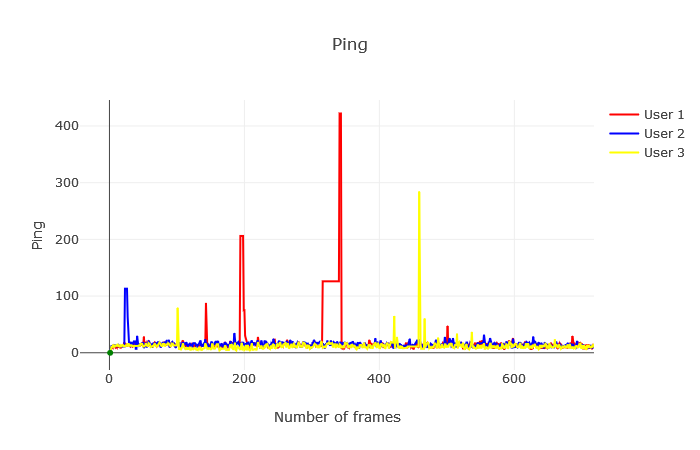
\includegraphics[width=7cm]{./images/ljoyping.png} % first figure itself
        \caption{Local joystick}
        \label{ljoyping}
    \end{minipage}\hfill
    \begin{minipage}{0.45\textwidth}
        \centering
        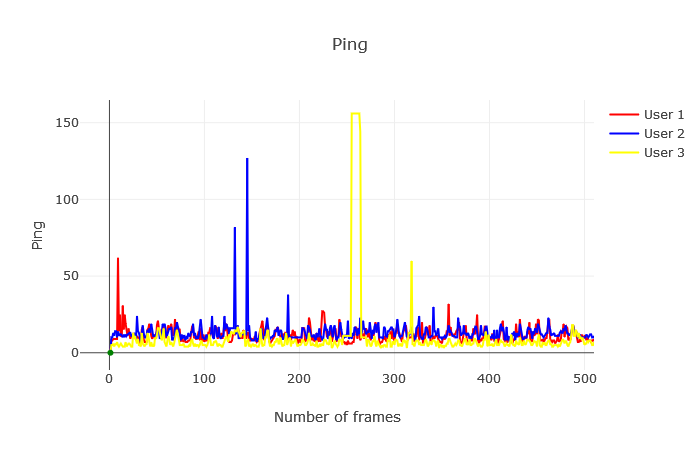
\includegraphics[width=7cm]{./images/ltouchping.png} % second figure itself
        \caption{Local touchpad}
        \label{ltouchping}
    \end{minipage}
\end{figure}

Overall, we can conclude that the joystick and the touchpad produce low ping and are therefore suitable for various purposes including gaming with very low lag. 


\subsection{Message rate}
The message rate captures the frequency of messages sent from the smartphone to the computer. Unlike with ping, the higher numbers are desirable here. When the rate is high it means we can achieve greater accuracy in control. \par 

Two different message rates are available: the user input message rate and the statistics message rate. The user input tracks how many messages per second have been sent from the smartphone controller by the player. 
The statistics message rate is the number of ping messages per second. \\

\subsubsection{Statistics message rate}
Statistic message rate is the number of stats type messages received in the last second. These are sent automatically from each device upon receiving a message of the same type from the computer. Figures on \ref{ljoys} and \ref{ltouchs} all three devices are connected locally. The rate is very high, ranging from 60 messages per second to 150 messages/s. The drops in the rate correspond to the ping spikes in figures \ref{ljoyping} and \ref{ltouchping}. \par

\begin{figure}[h!]
    \centering
    \begin{minipage}{0.45\textwidth}
        \centering
        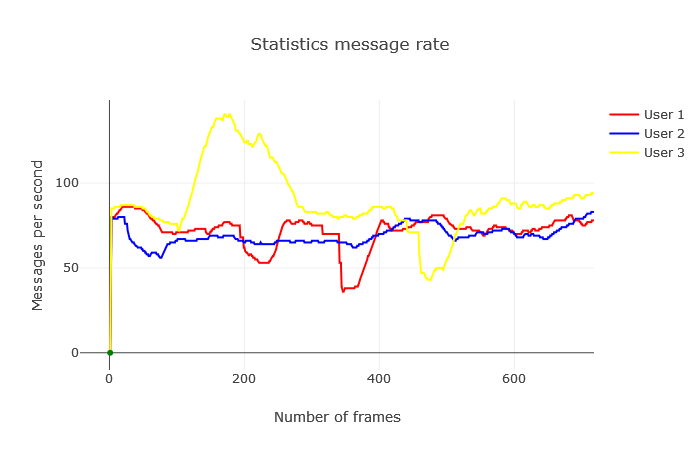
\includegraphics[width=7cm]{./images/ljoysmess.png} % first figure itself
        \caption{Local joystick, stats}
        \label{ljoys}
    \end{minipage}\hfill
    \begin{minipage}{0.45\textwidth}
        \centering
        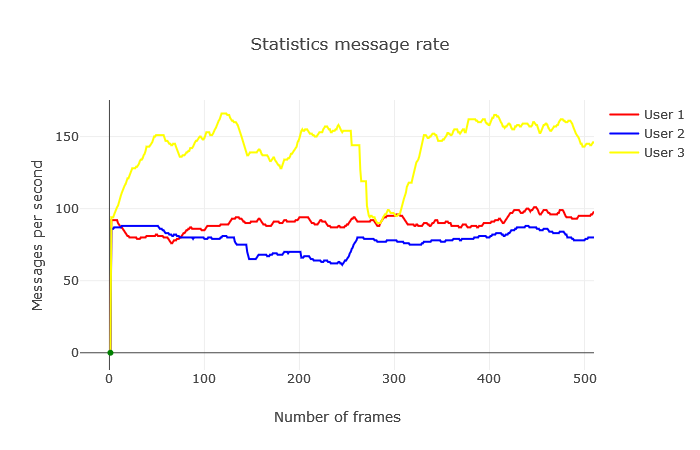
\includegraphics[width=7cm]{./images/ltouchsmess.png} % second figure itself
        \caption{Local touchpad, stats}
        \label{ltouchs}
    \end{minipage}
\end{figure}

Figures \ref{rjoys} and \ref{rtouchs} show the message rate for one local device and two remote devices. 
There is a clear difference in performance between the local red device and the two remote devices in blue and yellow. The red device sends between 60 and 70 messages per second while the blue and the yellow manage to send only about 30 to 35 messages. The higher ping was already demonstrated in the previous section hence, it was expected to see lower statistics message rate in yellow and blue devices. \par 
The performance can be influenced by both, distance and screen sharing. It is worth noting that despite the red device being local in \ref{rjoys}, the overall statistic message rate is lower than in the previous case, with all devices local \ref{ljoys}. This could be the effect of screen sharing while performing the evaluation.


\begin{figure}[h!]
    \centering
    \begin{minipage}{0.45\textwidth}
        \centering
        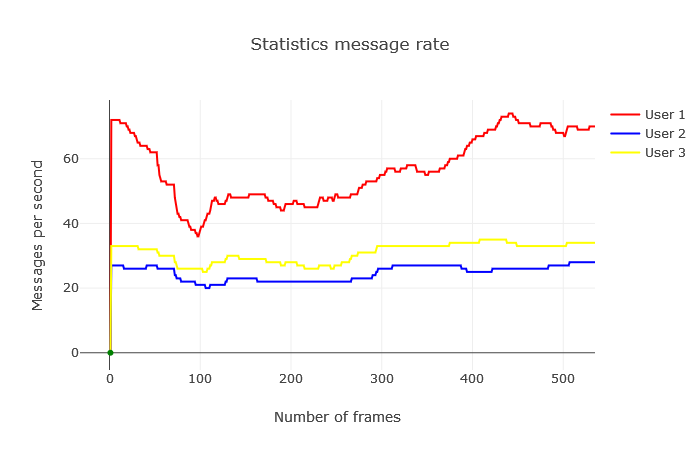
\includegraphics[width=7cm]{./images/rjoysmess.png} % first figure itself
        \caption{Remote joystick, stats}
        \label{rjoys}
    \end{minipage}\hfill
    \begin{minipage}{0.45\textwidth}
        \centering
        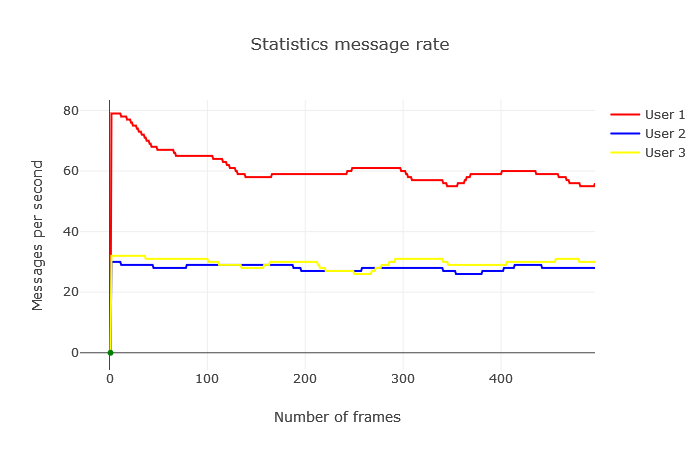
\includegraphics[width=7cm]{./images/rtouchsmess.png} % second figure itself
        \caption{Remote touchpad, stats}
        \label{rtouchs}
    \end{minipage}
\end{figure}



\subsubsection{User message rate} 
User message rate is calculated as the number of user-type messages received in the last second. The user rate could be compared to the mouse and gaming controllers’ polling rate. The polling rate is measured in Hz and it describes how often a controller reports its position or state to a computer or a console \cite{polling}. The standard polling rate for a mouse is 125Hz but a gaming mouse can have a rate of 500-1000Hz \cite{polling}. For PlayStation controllers the polling rate is 250Hz and for Xbox controllers it is about 124Hz \cite{game_polling}. \par

\begin{figure}[h!]
    \centering
    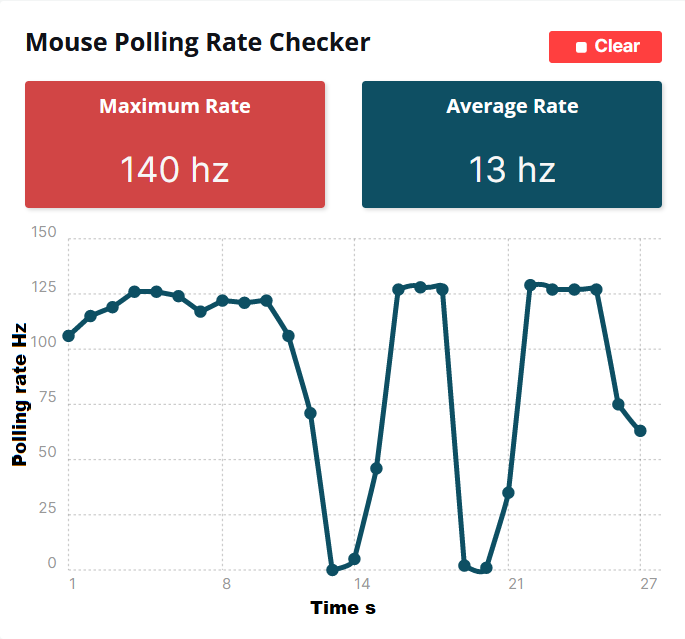
\includegraphics[width=7cm]{./images/mouse.png}
    \caption{Mouse polling rate}
    \label{fig:pollrate}
\end{figure}

Figure \ref{fig:pollrate} shows a sample polling rate of my mouse. The measurement was made with \href{https://devicetests.com/mouse-rate-test}{Device Tests}. The measurements are logged while moving the mouse in circles. The maximum rate I was able to achieve is 140 Hz with an average of around 125 Hz. During inactivity, the rate drops until it reaches 0 Hz which explains the drops in the graph and also the low average rate shown in the picture. \par

The controllers from SmartController follow similar logic when calculating the user message rate. The user message times are stored in an array that is periodically checked. All messages older than one second are deleted and the remaining messages are counted. During the inactivity period the rate drops as the old messages are gradually deleted. \par

Firstly, figures \ref{ljoyu} and \ref{ltouchu} show the user rate when all three devices are local. The maximum rate is around 60 Hz, that is there were 60 messages sent per second from each device. There is a lot of variability, this is created by the inactivity effect. It is unsurprising that with a local network all devices are performing similarly.  

\begin{figure}[h!]
    \centering
    \begin{minipage}{0.45\textwidth}
        \centering
        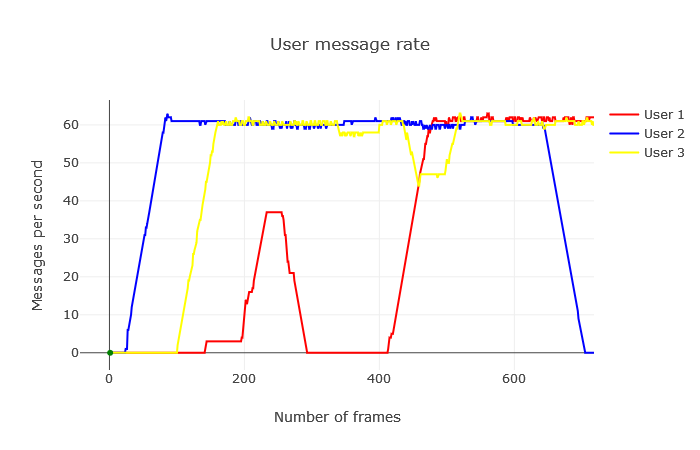
\includegraphics[width=7cm]{./images/ljoyumess.png} % first figure itself
        \caption{Local joystick, user}
        \label{ljoyu}
    \end{minipage}\hfill
    \begin{minipage}{0.45\textwidth}
        \centering
        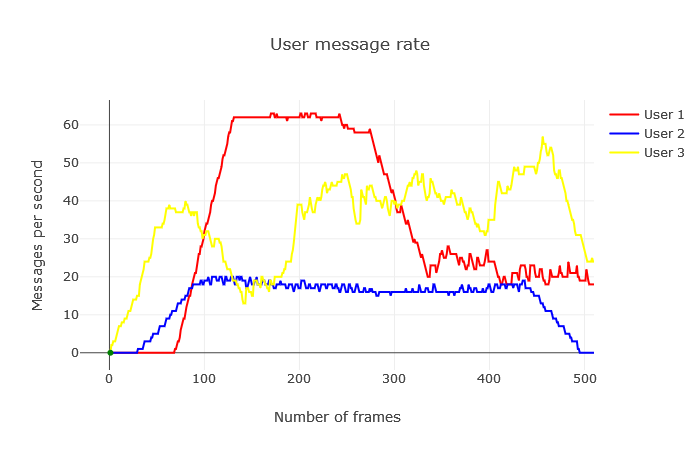
\includegraphics[width=7cm]{./images/ltouchumess.png} % second figure itself
        \caption{Local touchpad, user}
        \label{ltouchu}
    \end{minipage}
\end{figure}

It was more interesting to observe the effects of devices being used remotely on the user message rate. Unlike in statistics message rate, the smartphone does not wait for a confirming message from the computer, the user input messages are sent continuously as long as the controller is being used. \par

Figures \ref{rjoyu} and \ref{rtouchu} show that despite being used remotely, all of the devices were able to achieve a rate of at least 60 Hz. The yellow device stands out as its message rate is on average 30-40Hz higher than the other devices in both local and remote tests. \par

\begin{figure}[h!]
    \centering
    \begin{minipage}{0.45\textwidth}
        \centering
        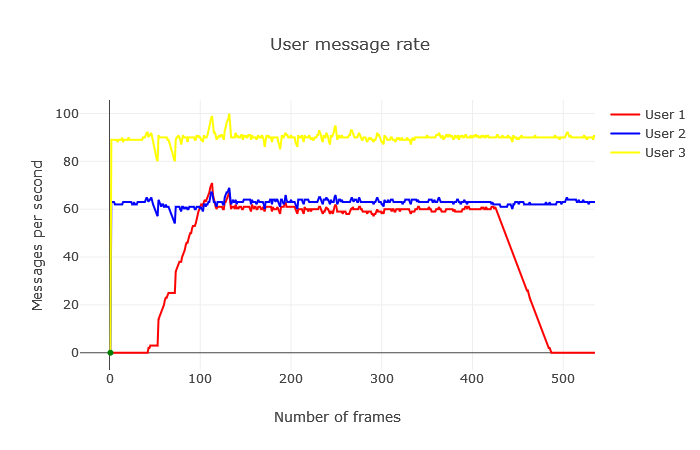
\includegraphics[width=7cm]{./images/rjoyumess.png} % first figure itself
        \caption{Remote joystick, user}
        \label{rjoyu}
    \end{minipage}\hfill
    \begin{minipage}{0.45\textwidth}
        \centering
        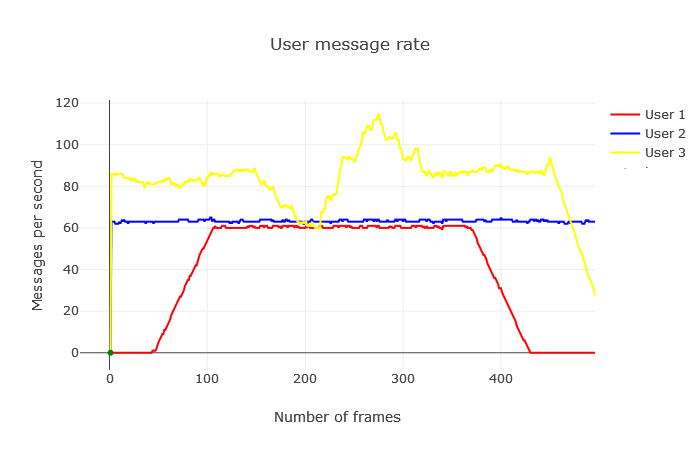
\includegraphics[width=7cm]{./images/rtouchumess.png} % second figure itself
        \caption{Remote touchpad, user}
        \label{rtouchu}
    \end{minipage}
\end{figure}

Overall, there appears to be a limit on the user rate message, it is unclear whether this is device-related or if it is associated with the peer-to-peer connection. The user message rate does not seem to be affected by remote use. In both cases, local and remote, the devices were able to send at least 60 messages per second. The user message rate of 60Hz is only half of an Xbox controller or a standard mouse. This is the reason why the SmartController offers two ways of accessing the data – state-based and event-based. Sometimes it is enough to have an event listener and react to the specific input. Many games and applications might refresh faster than the data event which could cause glitches, lag and could make the game hard to control. This problem was first discovered in the \href{https://emmapoliakova.github.io/WebRTCSmartphoneController/physics/physicsDemoV3.html}{block building demo}. In this demo, the touchpad is used to let the user pick up and drag a cube to a certain location. The cubes are part of a physics world; therefore, they are impacted by gravity. The cube is moved by scaling the coordinates from the smartphone screen to match the size of the computer screen. The cube's coordinates are then set to a particular location. When relying on the event-based mechanism the block would jump up and down in the gaps between the incoming messages, to the physics simulator this looked like the cube was being dropped repeatedly. Once the state-based movement was added, the dragging was smooth and easy to perform as during the message gaps the cube would simply retain its previous position. \par 
We can conclude that while the overall user message rate might be on the lower side, it works well in combination with the state-based actions. With this, the gaming or any other website controlling experience can be very smooth and the lower rate is unnoticeable. 


\subsection{Message throttle}
There might be a case where the user wished to regulate the number of user messages send. This might be for connection strength reasons or due to a high number of controllers connected to the same peer. For this purpose, it is possible to specify message throttle in milliseconds, i.e. how often a smartphone controller should send a message to the computer. The other messages will be discarded so this functionality should only be used when necessary. \par 

\begin{figure}[h!]
    \centering
    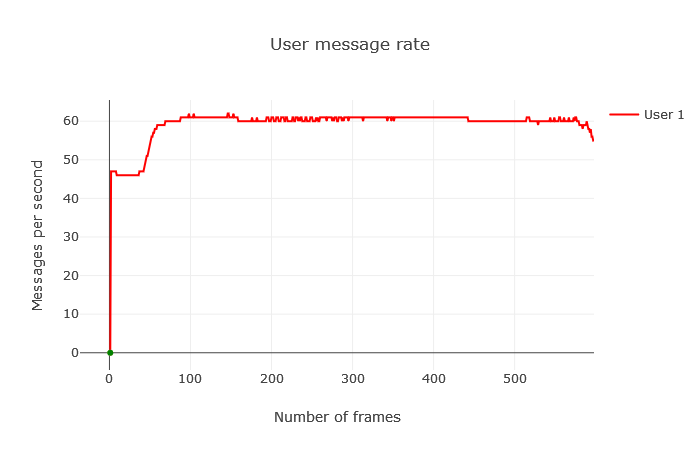
\includegraphics[width=10cm]{./images/nomthrot.png}
    \caption{No message throttle}
    \label{fig:nomthrot}
\end{figure}

Figure \ref{fig:nomthrot} shows the measurement of message rate from the prototype accelerometer with no throttle setting. With no limitation, the rate was 60 messages per second. In figure \ref{mthrot} the throttle is 20ms. The expected number of messages sent is now 50. However, with the throttle set, it is only 27-30 messages per second. In this case, the throttle effect seems to follow this pattern: \\ 
It takes about 17ms to send a message without restrictions: 1000ms / 60Hz = 17ms \\ 
Adding the delay of 20ms gives: 1000ms / (17ms + 20ms) = 27Hz. \par

\pagebreak

\begin{figure}[h!]
    \centering
        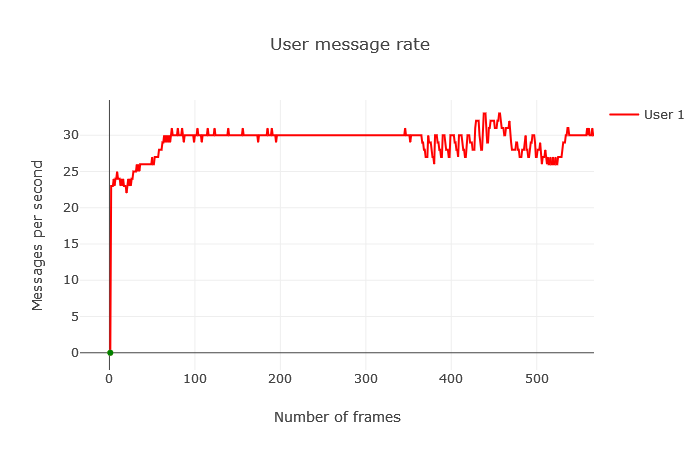
\includegraphics[width=10cm]{./images/mthrot.png} 
        \caption{Message throttle at 20ms}
        \label{mthrot}
\end{figure}

I compared the custom throttle with built-in JavaScript function setInterval also set to 20ms, figure \ref{setinterval}. It is interesting to observe that this function does not seem to be affected by the extra delay and sends 50 messages in a second as expected. 


\begin{figure}[h!]
        \centering
        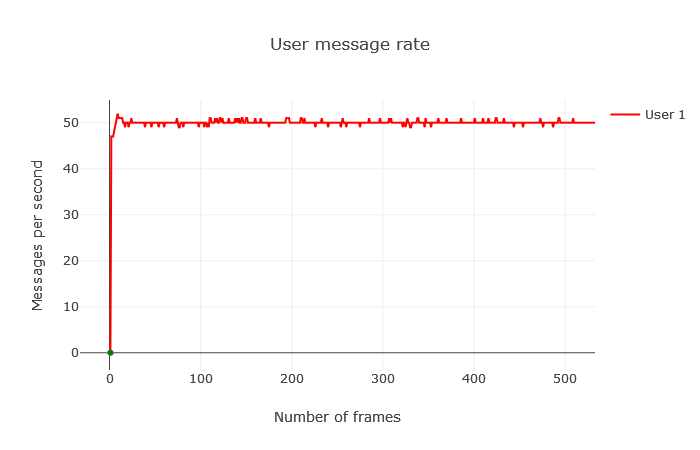
\includegraphics[width=10cm]{./images/setinterval.png} 
        \caption{Message throttle with setInterval}
        \label{setInterval}
\end{figure}


%==================================================================================================================================
\chapter{Conclusion}    

\section{Summary}
This project was focused on exploring the use of WebRTC and peer-to-peer communication to allow for the easy and free creation of smartphone controllers and accompanying websites. Users are now able to create peers without any prior knowledge of WebRTC. They can design their own controllers that will be tailored exactly to their needs.\par 
All the functional and non-functional requirements were fulfilled. This can be demonstrated through the documentation, the demos, and the evaluation. 
The main goal of this project was to make the process easier. The project was successful, when it first started the peer portion of the code would take around 50 lines ad was not very clear. Now it takes two lines for the computer side to create a peer and generate a QR code for the controller and similarly, when creating a smartphone controller, the user only needs two lines: one to make a peer, a second one to send a message. \par
The second important aim of this project was to support multiplayer integration by default. The project also achieved this, there is no need to specify how many connections there will be. The number of connections is mainly limited by the strength of broadband. 

\section{Reflection}
In terms of the programming itself, I think the project went well. I am happy with the design and implementation decisions that I made. This is largely thanks to the summer internship where I had time to get familiar with the technology and try different approaches. Therefore, I was heading into the project with a clear plan. The biggest obstacles I faced during the summer were the use of npm and Webpack. This saved me a lot of time later and I was able to focus on other areas, such as statistics functionality. \par
By working with other students I learned a lot about the development of an open-source library. If I was making another library, I would place more focus on early documentation. This is much needed for new users and it is the best way to explain how the code works. \par 
Another area I would prioritize is keeping a stable version of the code separate from the development version. This would be beneficial for the real-time users as publishing a version with possible errors would mean their projects would stop working too. \par


\section{Future work}
This project has a great potential to keep growing and evolving. There are features that could be perfected, such as working on greater device compatibility or providing more control over the QR code generation. While it is very difficult to offer a version that works for all browsers and devices, it would be good to have a mechanism for detecting the connection is not working in a given environment. It would inform the user that this is the case as well as log it for compatibility monitoring. \par
Some details could be improved on the controllers for a better user experience. These include stopping accidental refreshing of the page and taking screenshots and highlighting buttons when they are pressed longer. The refreshing of the page happens when the page is pulled down. This closes the original connection and created a new peer with a different ID. Stopping this from happening is especially important when players are added upon connection. This results in spawning of an extra character and possibly loss of the previous progress of the player. Highlighting of the buttons and screenshot taking with the use of three fingers are far less game-breaking but these events disturb the players. \par 
There are many smartphone sensors still unexplored. They could be a good base for new types of controllers. Using a microphone has a big potential as well as motion sensors. It might be worth revisiting the video streaming, either for hand tracking or basic object recognition. \par 
It is likely that there will be a paper written on the library and the games created with it so far during the summer.





%==================================================================================================================================
%
% 
%==================================================================================================================================
%  APPENDICES  

\begin{appendices}
%survey question\\
%nes graph\\
%table of demos\\
\chapter{Appendices}
\section{Table of demos}
This section lists all demos made during the summer internship and the level 4 project.\\

{
\begin{tabularx}{\textwidth} { 
  | >{\centering\arraybackslash}X |
 }
 \hline
 Summer internship demos: \\
 \hline
 \href{https://emmapoliakova.github.io/WebRTCSmartphoneController/demo/tinyPlatformer/index.html}{Platformer game} \\
  \hline
 \href{https://emmapoliakova.github.io/WebRTCSmartphoneController/demo/3dRacing.html}{3D racing} \\
  \hline
 \href{https://emmapoliakova.github.io/WebRTCSmartphoneController/physics/physicsDemoV3.html}{Physics simulator} \\
 \hline
\href{https://emmapoliakova.github.io/WebRTCSmartphoneController/physics/physicsDemoV4.html}{Physics simulator - multiplayer} \\
 \hline
\href{https://emmapoliakova.github.io/WebRTCSmartphoneController/handtracking/receiveVideo.html}{Hand tracking} \\
\hline
Level 4 project demos and documentation: \\
\hline
\href{https://smartcontrollerjs.github.io/Controllers/touchpad-receive.html}{Multiplayer touchpad} \\
\hline
\href{https://smartcontrollerjs.github.io/Controllers/controller-receive.html}{Nes controller arrows} \\
\hline
\href{https://smartcontrollerjs.github.io/Controllers/joystick-receive.html}{Joystick} \\
\hline
\href{https://smartcontrollerjs.github.io/Controllers/stats.html}{Statistics page} \\
\hline
\href{https://smartcontrollerjs.github.io/SmartController/}{Documentation} \\
\hline
\end{tabularx}
}


\pagebreak
\section{Nes controller statistics}
Figures from statistics evaluation for Nes controller. 
\begin{figure}[h!]
    \centering
    \begin{minipage}{0.45\textwidth}
        \centering
        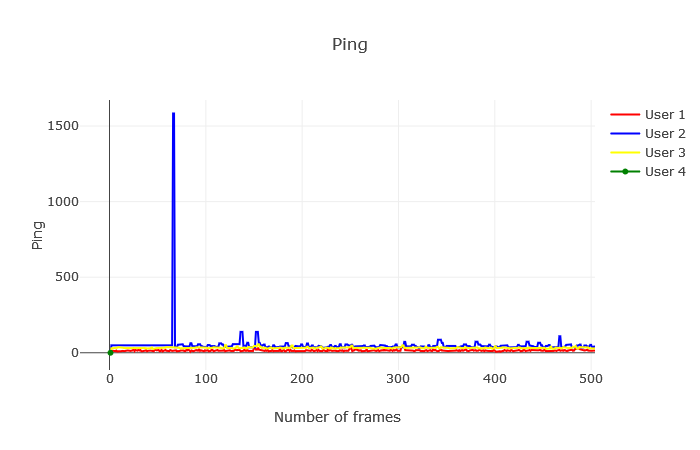
\includegraphics[width=7cm]{./images/rnessping.png} % first figure itself
        \caption{Remote Nes controller}
        \label{rnesping}
    \end{minipage}\hfill
    \begin{minipage}{0.45\textwidth}
        \centering
        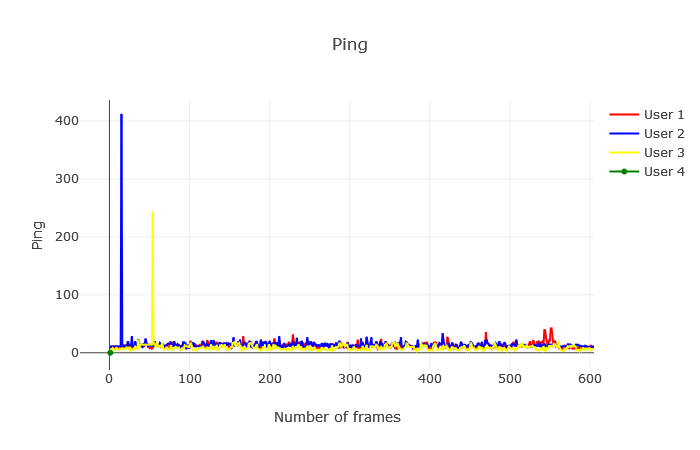
\includegraphics[width=7cm]{./images/lnessping.png} % second figure itself
        \caption{Local Nes controller}
        \label{lnesping}
    \end{minipage}
\end{figure}

\begin{figure}[h!]
    \centering
    \begin{minipage}{0.45\textwidth}
        \centering
        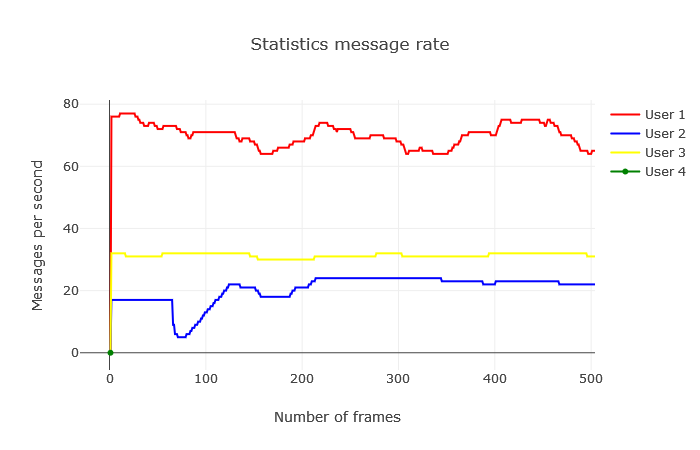
\includegraphics[width=7cm]{./images/rnessstats.png} % first figure itself
        \caption{Remote Nes controller, stats}
        \label{rnesstats}
    \end{minipage}\hfill
    \begin{minipage}{0.45\textwidth}
        \centering
        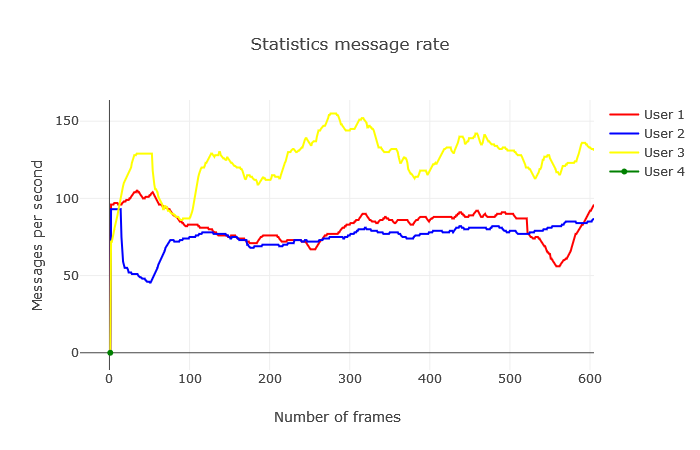
\includegraphics[width=7cm]{./images/lnessstats.png} % second figure itself
        \caption{Local Nes controller,stats}
        \label{lnesstats}
    \end{minipage}
\end{figure}

\begin{figure}[h!]
    \centering
    \begin{minipage}{0.45\textwidth}
        \centering
        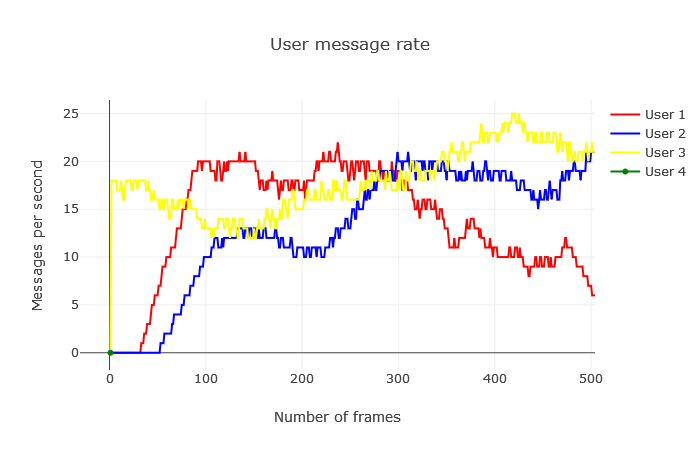
\includegraphics[width=7cm]{./images/rnessuser.png} % first figure itself
        \caption{Remote Nes controller, user}
        \label{rnesuser}
    \end{minipage}\hfill
    \begin{minipage}{0.45\textwidth}
        \centering
        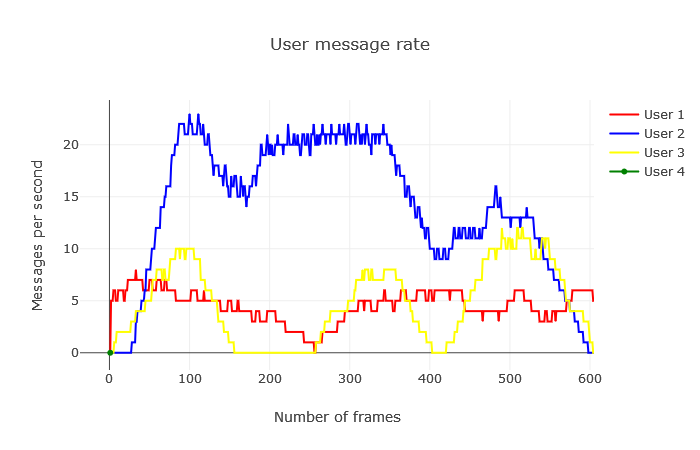
\includegraphics[width=7cm]{./images/lnessuser.png} % second figure itself
        \caption{Local Nes controller, user}
        \label{lnesuser}
    \end{minipage}
\end{figure}

\pagebreak
\section{Ethics checklist}
Bellow is the signed ethics checklist: 

\begin{figure}[h!]
    \centering
    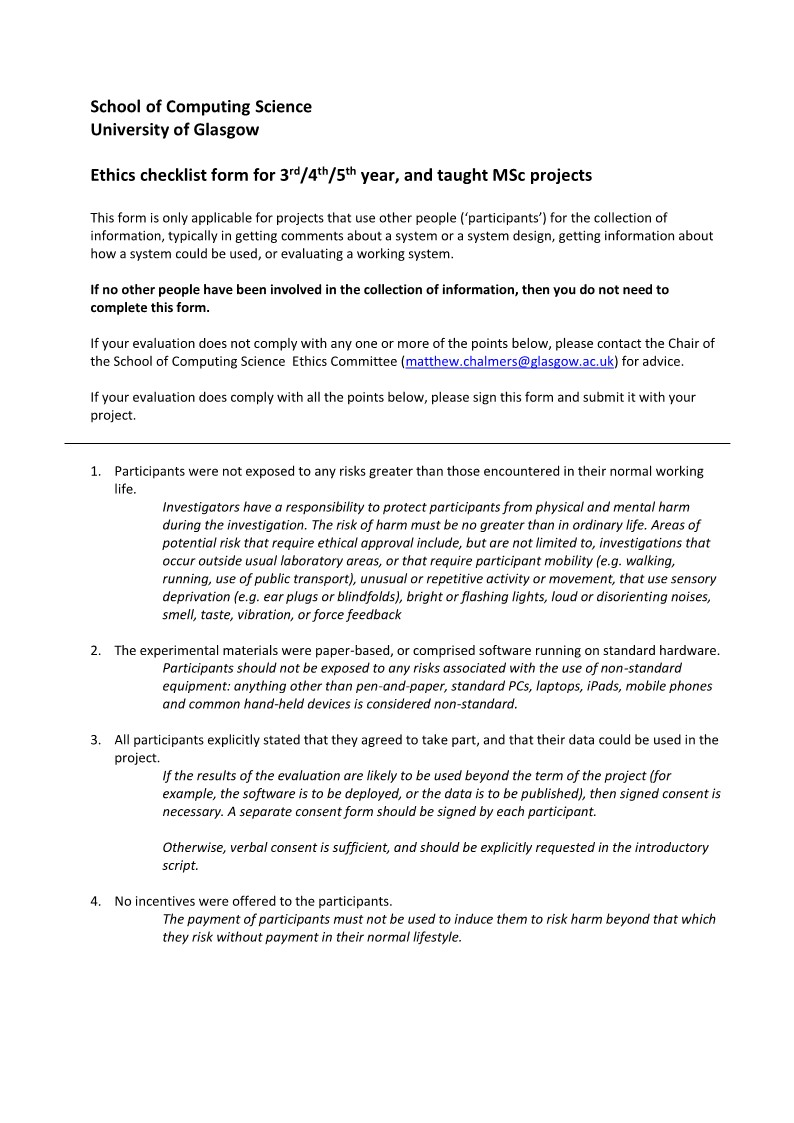
\includegraphics[width=13.5cm]{./images/ethics1.jpg}
    \caption{Ethics checklist part 1}
\end{figure}
\pagebreak

\begin{figure}[h!]
    \centering
    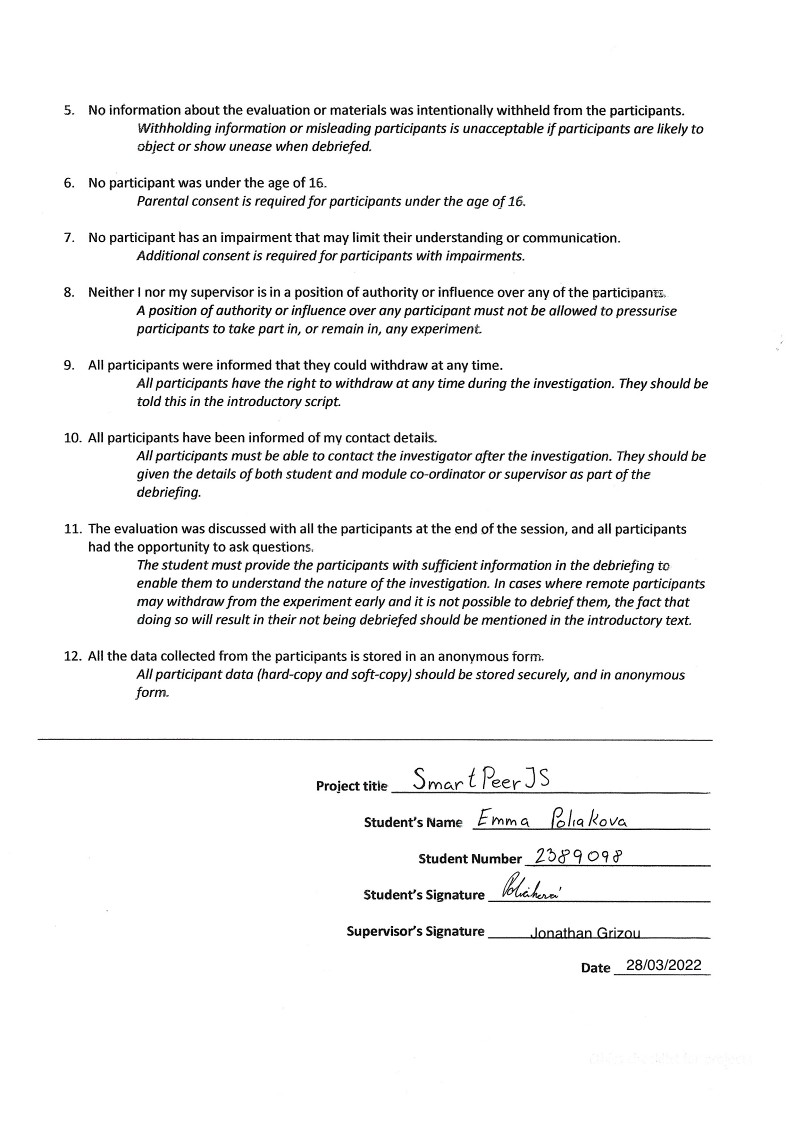
\includegraphics[width=13.5cm]{./images/ethics2.jpg}
    \caption{Ethics checklist part 2}
\end{figure}

\pagebreak

\section{Library name survey}
The following survey was conducted to find out the optimal name and keywords for the library: 

\begin{figure}[h!]
    \centering
    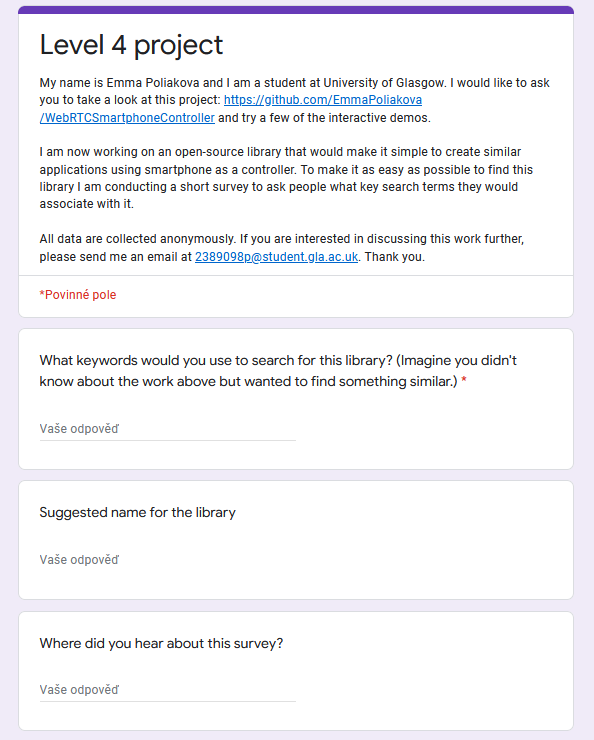
\includegraphics[width=14cm]{./images/survey.png}
    \caption{Library name survey}
\end{figure}


\end{appendices}

%==================================================================================================================================
%   BIBLIOGRAPHY   

% The bibliography style is agsm (Harvard)
% The bibliography always appears last, after the appendices.

\bibliographystyle{agsm}

% Force the bibliography not to be numbered
\renewcommand{\thechapter}{0} 
\bibliography{l4proj}

\end{document}
